% Archive of Applied Mechanics authoring CANDIDATE (not yet submission-ready).
% Editorial transformation of ../../main.tex (frozen, verified scientific baseline).
% Requires the OFFICIAL Springer Nature sn-jnl.cls and sn-mathphys-num.bst.
% Place official template files beside this manuscript or on the LaTeX search path.
% Journal guidance currently conflicts on [iicol] vs single-column;
% this first build deliberately uses the safer single-column layout.
\documentclass[pdflatex,sn-mathphys-num]{sn-jnl}
\usepackage{amsmath,amssymb,bm,booktabs}
\usepackage{graphicx}
\usepackage{placeins,needspace}
\usepackage{subcaption}
\captionsetup[subfigure]{font=footnotesize,skip=3pt}
\graphicspath{{../../}}
% The original 31 approved vector PDFs remain in ../../figures/.
% For the journal upload, copy/flatten graphics into the upload archive.

\newcommand{\qmix}{q_{\mathrm{K}}}
\newcommand{\dd}{\mathrm{d}}
% BEGIN AUDITED DATA: populated by sync_manuscript_data.py
% Snapshot: cfdf0f110010d688a4e3c48f6d88a00fd17dc698; no P24 physical data.
% Evidence JSON SHA256: db7c5908e2cad5c749c7914f4eb742b28d1d404b4124a03107f35b94ad013bd3
\newcommand{\PlateAMM}{300}
\newcommand{\PlateBMM}{100}
\newcommand{\HoleCxMM}{170}
\newcommand{\HoleCyMM}{-20}
\newcommand{\HoleRMM}{30}
\newcommand{\PhiStar}{-1.5606}
\newcommand{\MouthX}{0.199989}
\newcommand{\MouthY}{-0.0208170}
\newcommand{\NormalX}{0.999629}
\newcommand{\NormalY}{-0.0272345}
\newcommand{\PeakStress}{3.7141}
\newcommand{\LoadFactor}{80.774}
\newcommand{\LastXMM}{291.840}
\newcommand{\LastYMM}{-25.579}
\newcommand{\LSLengthMM}{84.15}
\newcommand{\LastLigamentMM}{8.16}
\newcommand{\MinimumTheta}{-3.646}
\newcommand{\MaxCODError}{0.01024}
\newcommand{\CODQuadMin}{0.6204}
\newcommand{\CODQuadMax}{0.6225}
\newcommand{\CODNearZeroPercent}{26.3}
\newcommand{\CODNearZeroTurnDiff}{0.00245}
\newcommand{\SyntheticRelativeError}{3.86\times10^{-8}}
\newcommand{\MaxTrueResidual}{1.00\times10^{-10}}
\newcommand{\CharacteristicRows}{$P_{1}$ & 4 & 0.36648 & $4.198\times10^{-6}$ & $1.146\times10^{-5}$ & 0.0000 & -0.00131 \\
$P_{17}$ & 68 & 0.78679 & $2.548\times10^{-3}$ & $3.239\times10^{-3}$ & -2.4444 & -0.37115 \\
$P_{21}$ & 84 & 0.96631 & $7.860\times10^{-5}$ & $8.134\times10^{-5}$ & -3.6366 & -0.00932 \\
$P_{22}$ & 88 & 1.0667 & $-2.284\times10^{-3}$ & $-2.142\times10^{-3}$ & -3.6460 & +0.24541 \\
$P_{23}$ & 92 & 1.2444 & $-6.780\times10^{-3}$ & $-5.449\times10^{-3}$ & -3.4006 & +0.62435 \\}
% END AUDITED DATA

\begin{document}
\title[LEFM crack trajectory from a circular hole]{Incremental LEFM Prediction of a Crack Trajectory from a Circular Hole}
\author*[1]{\fnm{Danylo} \sur{Selivanov}}
\email{fract@inmech.kyiv.ua}
\affil*[1]{\orgname{S.P. Timoshenko Institute of Mechanics},
  \orgdiv{National Academy of Sciences of Ukraine}, \city{Kyiv}, \country{Ukraine}}

\abstract{
Predicting a crack trajectory from an initially uncracked circular hole
requires linking the initiation state to a sequence of mixed-mode
crack-tip solutions. We consider this problem within quasi-static linear
elastic fracture mechanics. The initiation point is selected by the
maximum tensile tangential stress on the hole boundary, and the
first segment follows the outward material-side normal. Subsequent
directions are determined by the maximum tangential stress criterion
using interaction-integral stress-intensity factors evaluated for the
complete current crack geometry. Prescribed-field checks,
crack-opening-displacement comparisons, and a centered-hole
symmetry control assess the extraction and direction-selection
procedures. Independently propagated exterior-mesh and
structured-tip calculations test the sensitivity of the resulting
trajectory. In the asymmetric case, the signed mode-mixity ratio
reaches a positive maximum and then changes sign, reversing the
incremental turning sense while the opening-mode intensity
continues to increase under fixed remote traction. Independently
propagated 4-, 2-, and 1-mm paths, refined together with their
numerical length scales, exhibit contracting geometric and
directional differences and nearly constant increment-normalized
turning measures. The characteristic turning sequence persists under the tested mesh
changes; coupled refinement reveals trends in mode mixity and
turning density without isolating the effect of the increment.
}
\keywords{crack trajectory, circular hole, linear elastic fracture mechanics,
 maximum tangential stress, mode mixity, interaction integral}
\hypersetup{%
  pdftitle={Incremental LEFM Prediction of a Crack Trajectory from a Circular Hole},%
  pdfauthor={Danylo Selivanov}%
}
\maketitle

\section{Introduction}
The initiation and subsequent propagation of a crack at a circular hole
are related but distinct fracture-mechanics problems. Stress-intensity
factors (SIFs) for prescribed radial and inclined hole-edge cracks have been
studied since the classical work of Bowie~\cite{Bowie1956}; mixed-mode
solutions for finite plates~\cite{WooWangCheung1989} and weight-function
methods~\cite{XuEtAl2018} have extended their evaluation to other
geometries and loading conditions. For an initially uncracked hole,
the initiation site must first be determined from the stress field or a
fracture criterion. Finite-fracture-mechanics analyses have examined
both symmetric and asymmetric initiation~\cite{SaporaEtAl2018} and
subsequent growth stability under biaxial loading
\cite{SaporaCornetti2018}. Selection of the initiation site, however,
does not determine the path followed by a crack of finite length.

Once the first segment has formed, each change in crack direction
alters the geometry and hence the mixed-mode field at the advancing
tip. The maximum tangential stress (MTS) criterion of Erdogan and
Sih~\cite{ErdoganSih1963} supplies a local direction rule in terms of
the opening- and sliding-mode stress-intensity factors,
$K_{\mathrm{I}}$ and $K_{\mathrm{II}}$, respectively. Such criteria
have long been incorporated into finite-element procedures with
successive remeshing; Bouchard et al.~\cite{BouchardEtAl2003},
for example, compared alternative mixed-mode criteria in an
automatic propagation framework. A cohesive-zone description
instead resolves the fracture process zone rather than retaining
an ideally sharp singular tip. Recent potential-based cohesive
calculations~\cite{BogdanovSelivanov2026} provide a useful
comparison with classical elastic kink predictions, although the
present study is confined to linear elastic fracture mechanics
(LEFM) and direction selection for prescribed crack extensions.

Hole-induced crack deflection has also been investigated using
several computational approaches. Wang et al.~\cite{WangMeguidPapanikos1999}
studied curved cracks emanating from adjacent holes; boundary-element
methods have been applied to multiple cracks in perforated
solids~\cite{LiuLiXie2017}. Fang et al.~\cite{FangEtAl2020}
combined adaptive extended isogeometric analysis with an
interaction integral for cracks interacting with holes and voids,
and compared trajectories obtained with two extension increments.
Related studies include incremental remeshing for cracks from
blasting holes~\cite{YangEtAl2020}, boundary-cracklet
propagation in perforated plates~\cite{AhmedEtAl2021}, and
finite-element simulations of hole-induced deflection
\cite{AlshoaibiFageehi2022}. These investigations demonstrate
the range of available methods, but visual agreement between
trajectories alone does not quantify the sensitivity of their
successive direction updates.

Sensitivity to SIF extraction matters because the calculated
intensities determine the next crack geometry and thus influence
all subsequent elastic solutions. Interaction integrals offer
a means of separating the mixed-mode contributions
\cite{YauWangCorten1980}, while displacement-extrapolation
estimates are sensitive to near-tip element arrangements
\cite{GuineaPlanasElices2000}. Comparisons of extraction
procedures have emphasized the advantages of integral
methods~\cite{CourtinEtAl2005} and their dependence on
adequate finite-element resolution~\cite{QianEtAl2016}.
Mixed-mode assessments have likewise examined the response
of interaction-integral estimates to discretization choices
\cite{GhafooriAhangarVerreman2019}. For a recursively generated
path, such local extraction differences can also alter the
later crack geometries. Accuracy checks for a prescribed tip
must therefore be distinguished from comparisons of
independently propagated trajectories.

We investigate this question for a single crack initiating
at an asymmetric circular hole in a finite plate. The maximum
tensile tangential stress of the uncracked-hole solution determines
the initiation point and its outward material-side normal.
Only the first crack segment is prescribed along that normal.
At each subsequent step, the current elastic boundary-value
problem is solved for the complete accumulated crack geometry,
and the next direction is selected from the current-tip SIFs
using the MTS criterion. Our objective is to identify which features of the
calculated trajectory persist under the tested changes
in SIF extraction and discretization, rather than
to introduce a new fracture criterion.

% Permit small emergency stretch only within this paragraph.
\begingroup
\setlength{\emergencystretch}{1em}
The assessment combines prescribed-field and fixed-geometry
checks with independent crack-path calculations. Interaction-integral
SIFs are compared with crack-opening-displacement (COD)
extrapolations from the same computed displacement field; a
centered-hole control probes reflection symmetry and the local
one-step angular response. Independently propagated paths
then test changes in exterior-mesh density and structured-tip
resolution. A separate family with 4-, 2-, and 1-mm increments
also refines the numerical length scales, so that it examines
coupled increment/discretization sensitivity rather than the
increment in isolation. We examine the positive maximum and subsequent sign reversal
of mode mixity, their effect on the MTS turning direction,
and the behavior of increment-normalized turning measures
under coupled refinement.
\par\endgroup

Sections~\ref{sec:problem} and \ref{sec:recurrence} define the
physical problem and the incremental MTS construction.
Sections~\ref{sec:numerics} and \ref{sec:results} present the
numerical assessment and crack-trajectory results, followed
by the physical interpretation, limitations, and conclusions
in Sections~\ref{sec:discussion} and \ref{sec:conclusions}.

\section{Problem formulation}
\label{sec:problem}
\subsection{Geometry, material, and loading}
Figure~\ref{fig:geometry-loading} introduces the plate geometry, the
coordinate conventions, and the applied loading. The specimen has
width $2A$ and height $B$, with a circular hole of radius $R$ whose
center is denoted in the schematic by $(x_{\mathrm{c}},y_{\mathrm{c}})$, where $x_{\mathrm{c}}$
and $y_{\mathrm{c}}$ are the coordinates measured from the lower-left corner.
The computational Cartesian frame has its origin at the midpoint of
the left edge, with $x$ pointing right and $y$ upward. Its rectangular
domain is
\[
  \Omega_{\mathrm{rect}}=[0,2A]\times[-B/2,B/2].
\]
In this frame the hole center is $(x_{\mathrm{c}},y_{\mathrm{c}}-B/2)$; no separate symbol
for the shifted center ordinate is needed.
The curved line emerging from the hole illustrates an admissible
crack path; it is schematic and does not prescribe the computed
trajectory. The initiation point $P_0$ is selected from the
uncracked-hole solution, and only the first crack direction is
prescribed. Subsequent directions follow from the current-tip SIFs.

% Figure environment maintained inline in main.tex; graphics remain separate PDFs.
\begin{figure}[htbp]
  \centering
  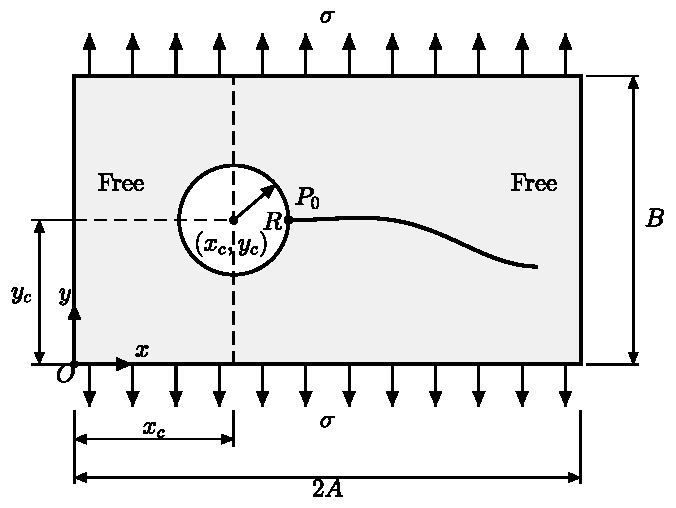
\includegraphics[width=0.78\textwidth]{figures/geometry_loading/specimen_geometry.pdf}
  \caption{Plate geometry and tensile loading. Hole-center coordinates
  $(x_{\mathrm{c}},y_{\mathrm{c}})$ are measured from the lower-left corner;
  the computational ordinate is shifted by $-B/2$. The horizontal
  edges carry outward tensile tractions of magnitude $\sigma$,
  while the remaining boundaries and crack faces are traction-free.
  The curved crack is schematic; dimensions are not to scale.}
  \label{fig:geometry-loading}
\end{figure}

At step $k$, $\Omega_k$ is the material domain outside the hole and the
retained crack $\Gamma_k$, with distinct upper and lower crack faces.
The material is homogeneous, isotropic, and linearly elastic,
with Young's modulus $E$ and Poisson's ratio $\nu$, under plane
strain. For the crack geometry $\Gamma_k$ ending at $P_k$, the
displacement field $\bm u$, strain tensor $\bm\varepsilon$, and stress
tensor $\bm\sigma$ satisfy
\begin{align}
 \nabla\!\cdot\bm{\sigma}&=\bm0 &&\text{in }\Omega_k,\label{eq:equilibrium}\\
 \bm{\varepsilon}&=\tfrac12(\nabla\bm u+\nabla\bm u^{\mathsf T}),\qquad
 \varepsilon_{33}=0,\label{eq:strain}\\
 \bm{\sigma}&=2\mu\bm{\varepsilon}
       +\lambda\,\operatorname{tr}(\bm{\varepsilon})\bm I,
 \quad \mu=\frac{E}{2(1+\nu)},\quad
 \lambda=\frac{E\nu}{(1+\nu)(1-2\nu)}.\label{eq:constitutive}
\end{align}
Here $\bm I$ is the identity tensor, and $\mu$ and $\lambda$ are the
shear modulus and first Lam\'e coefficient, both with stress units.
Uniform outward tensile tractions act on the horizontal edges, in the
directions indicated by the arrows in Fig.~\ref{fig:geometry-loading}.
Their unsigned magnitude is $\sigma>0$, as in the drawing. The traction
vectors on the upper and lower edges are $(0,\sigma)$ and
$(0,-\sigma)$, respectively. The vertical sides, hole boundary, and
crack faces are traction free. Rigid-body motions are removed by imposing
$u_x=u_y=0$ at the lower-left corner and $u_y=0$ at the lower-right
corner. There are no body forces.

For fixed geometry, positive scaling of $\sigma$ scales both SIFs
equally, preserving their ratio and the MTS direction. The present
formulation predicts the direction of imposed quasi-static increments,
not a load-versus-time crack-growth history.

\subsection{Stress-selected initiation and the frozen frame}
The uncracked-hole elastic field supplies the tangential boundary stress
$\sigma_{tt}(\phi)$, where $\phi$ is measured counterclockwise from the
positive Cartesian $x$ direction. Its maximum tensile value selects the
initiation point; the numerical boundary evaluation is described in
Section~\ref{sec:numerics}. Let $\sigma_{\mathrm{ini}}$ denote the
prescribed tensile-stress threshold for initiation, not a cohesive
strength. The dimensionless initiation load multiplier
$\Lambda_{\mathrm{ini}}$ is the ratio of this threshold to the maximum
tensile stress under the reference loading; it is distinct from the
first Lam\'e coefficient $\lambda$. The initiation rule is
\begin{equation}
 \phi_* = \mathop{\operatorname{arg\,max}}_\phi
      \sigma_{tt}^{+}(\phi;\sigma),\qquad
 \Lambda_{\mathrm{ini}}=
      \frac{\sigma_{\mathrm{ini}}}{\max_\phi\sigma_{tt}^{+}(\phi;\sigma)},
 \quad \sigma_{tt}^{+}=\max(\sigma_{tt},0).\label{eq:initiation}
\end{equation}
The fitted angle $\phi_*$ specifies the initiation point and the
outward material-side radial normal:
\begin{equation}
 P_0=\begin{bmatrix}x_{\mathrm{c}}+R\cos\phi_*\\
                     y_{\mathrm{c}}-B/2+R\sin\phi_*
     \end{bmatrix}.
 \label{eq:mouth}
\end{equation}
The stress-based initiation condition supplies the location and the
corresponding load multiplier; it is not reused as a growth or arrest
criterion along the crack. No cohesive traction--separation law is
introduced in the present LEFM formulation.

The frozen basis is
\begin{equation}
 \bm n_{\mathrm{mat}}=
  \begin{bmatrix}\cos\phi_*\\\sin\phi_*\end{bmatrix},
 \qquad
 \bm t=\begin{bmatrix}-n_{\mathrm{mat},y}\\n_{\mathrm{mat},x}\end{bmatrix}.
 \label{eq:frozenframe}
\end{equation}
The normal points radially out of the hole and into the material; $\bm t$
is its counterclockwise rotation. All absolute crack angles $\theta_k$
below are measured relative to this frozen normal, not to the global
$x$ axis. Its global orientation is $\phi_*+\theta_k$; translating the
coordinate origin does not change this angle. With increment length $\Delta a$, the initial direction and
first segment are prescribed by
\begin{equation}
 \theta_1=0,\qquad
 P_1=P_0+\Delta a\,\bm n_{\mathrm{mat}}.\label{eq:first}
\end{equation}
The initiation point and frame remain frozen for subsequent increments.
The study treats one active crack; competing subsequent initiation sites
are outside its scope.

\section{Incremental crack-path formulation}
\label{sec:recurrence}
\subsection{Current-tip frame and stress-intensity factors}
At the current tip $P_k$, the local forward unit vector
$\bm e_1^{(k)}=(P_k-P_{k-1})/\Delta a$ follows the last crack
segment; $\bm e_2^{(k)}=(-e_{1y}^{(k)},e_{1x}^{(k)})$ is its
counterclockwise normal. Thus the local frame follows the current
tip direction rather than the chord connecting the crack mouth to the
tip. With $x_1$ and $x_2$ measured along these vectors and $r>0$
measured directly ahead of the tip, the opening- and sliding-mode
stress-intensity factors are defined by
\begin{equation}
 K_{\mathrm{I}}^{(k)}=\lim_{r\to0^+}\sqrt{2\pi r}\,\sigma_{22}(r,0),
 \qquad
 K_{\mathrm{II}}^{(k)}=\lim_{r\to0^+}\sqrt{2\pi r}\,\sigma_{12}(r,0).
 \label{eq:sifdefinition}
\end{equation}
Here $\sigma_{22}$ and $\sigma_{12}$ are the stress components in
the current-tip frame. The signed mode-mixity ratio is defined for
positive opening-mode intensity by
\begin{equation}
 q_{\mathrm{K}}^{(k)}
 =\frac{K_{\mathrm{II}}^{(k)}}{K_{\mathrm{I}}^{(k)}},
 \qquad K_{\mathrm{I}}^{(k)}>0.
 \label{eq:mode-mixity}
\end{equation}
This dimensionless ratio has the sign of the sliding-mode intensity.
Both stress-intensity factors are extracted from an elastic solution
that retains the complete preceding crack geometry.

\subsection{The implemented MTS rule}
The maximum tangential stress (MTS) criterion determines the direction
of a new segment relative to the preceding one. Let $\alpha$ be the
counterclockwise turning angle in local polar coordinates centered at
the crack tip, and write $c=\cos(\alpha/2)$ and
$s=\sin(\alpha/2)$. The functions $S(\alpha)$ and $T(\alpha)$ are
the angular amplitudes of the leading circumferential normal stress
and radial--circumferential shear stress, respectively:
\begin{align}
 S(\alpha)&=K_{\mathrm{I}}^{(k)}c^3
             -3K_{\mathrm{II}}^{(k)}s c^2,\label{eq:stt}\\
 T(\alpha)&=K_{\mathrm{I}}^{(k)}s c^2
             +K_{\mathrm{II}}^{(k)}c(1-3s^2).
 \label{eq:trt}
\end{align}
Both stresses have the common singular factor $1/\sqrt{2\pi r}$.
Since $S'(\alpha)=-3T(\alpha)/2$, the stationary circumferential-stress
directions satisfy $T(\alpha)=0$. The numerical procedure selects the
tensile root continuously connected to straight extension as
$K_{\mathrm{II}}^{(k)}\to0$. The accepted states have positive opening
intensity and small turning angles; the implemented root search and
its safeguards are unchanged.

For $|q_{\mathrm{K}}^{(k)}|\ll1$, expansion on this branch gives
\begin{equation}
 \alpha_{\mathrm{MTS}}
 =-2q_{\mathrm{K}}^{(k)}
  +\frac{14}{3}\bigl(q_{\mathrm{K}}^{(k)}\bigr)^3
  +O\bigl((q_{\mathrm{K}}^{(k)})^5\bigr),
 \label{eq:mts-small-mixity}
\end{equation}
where the angle is in radians. In particular, positive mode mixity
produces clockwise turning in the adopted frame. This expansion is
used for interpretation, whereas the reported trajectories use the
unapproximated MTS root.

\subsection{Finite-increment recurrence}
The unit direction of a segment is expressed in the frozen initiation
basis. The incremental turning angle, the absolute direction of the new
segment, and its tip position satisfy
\begin{align}
 \bm e(\theta)&=\cos\theta\,\bm n_{\mathrm{mat}}
                 +\sin\theta\,\bm t,\label{eq:direction}\\
 \Delta\theta_{k+1}
   &=\alpha_{\mathrm{MTS}}(K_{\mathrm{I}}^{(k)},K_{\mathrm{II}}^{(k)}),
     \label{eq:turn}\\
 \theta_{k+1}&=\theta_k+\Delta\theta_{k+1},\label{eq:angleupdate}\\
 P_{k+1}&=P_k+\Delta a\,\bm e(\theta_{k+1}).\label{eq:pointupdate}
\end{align}
Here $\theta_k$ is measured relative to the fixed outward normal at
the initiation point. The accumulated crack-path length, measured from the initiation
point $P_0$, is $a_k=k\Delta a$. Throughout the numerical results,
$a$ denotes this length rather than the horizontal coordinate of the crack tip. The accepted
elastic solution for each current geometry determines the following
segment, so the propagation history enters recursively through the
boundary-value problem.

The turning density $\Delta\theta_{k+1}/\Delta a$ is the signed
angle change per unit extension. It does not represent the
pointwise curvature of the polygonal crack, whose direction is
discontinuous at its vertices. Consider instead a family of
decreasing increments and suppose that the computed polygons
approach an arc-length-parametrized curve $\bm r(a)$ with a
differentiable tangent angle $\theta(a)$. If, in addition, their
discrete turning densities converge at corresponding crack lengths
to the signed curvature $\dd\theta/\dd a$, the small-turn
MTS expansion implies
\begin{equation}
 \frac{q_{\mathrm{K}}^{(k)}}{\Delta a}
 =-\frac12\frac{\Delta\theta_{k+1}}{\Delta a}
  +O((\Delta a)^2)
 \longrightarrow-\frac12\frac{\dd\theta}{\dd a}.
 \label{eq:curvature-mts}
\end{equation}
Indeed, a bounded turning density implies
$\Delta\theta_{k+1}=O(\Delta a)$, and therefore
$q_{\mathrm{K}}^{(k)}=O(\Delta a)$ on the selected small-turn
branch. Positive curvature corresponds to counterclockwise
turning, hence to negative mode mixity. This relation is a
conditional smooth-path interpretation, not a convergence
theorem: convergence of polygonal positions alone does not ensure
convergence of the turning densities, and numerical SIF extraction
must resolve mode mixity at the scale of $\Delta a$.

\section{Numerical implementation and verification}
\label{sec:numerics}
The computation begins with stress-selected initiation and proceeds by
solving successive cracked geometries with a structured near-tip mesh.
We describe the interaction-integral and crack-opening-displacement
(COD) extractions, the numerical acceptance criteria, and the
mesh configurations used to assess their sensitivity. The subsequent
tests address two distinct questions. Prescribed fields and fixed
crack geometries examine SIF extraction without changing the path,
whereas independently propagated calculations reveal how differences
in the discretization affect successive crack directions. A coupled
4/2/1-mm refinement study and a centered-hole symmetry control
complete the numerical assessment. The trajectory results are
presented in Section~\ref{sec:results}.

\subsection{Numerical parameters and initiation state}
\label{sec:numerical-parameters}
For the computations, $2A=\PlateAMM$ mm, $B=200$ mm, and
$R=\HoleRMM$ mm. The center is $(x_{\mathrm{c}},y_{\mathrm{c}})=(170,80)$ mm in the
lower-left convention of Fig.~\ref{fig:geometry-loading}; in the
midheight computational frame it is
$(\HoleCxMM,\HoleCyMM)$ mm. The material constants are
$E=210$ GPa and $\nu=0.30$ (plane strain). The reference
tensile traction is $\sigma=1$ MPa, and the tensile initiation
threshold is $\sigma_{\mathrm{ini}}=300$ MPa.

The uncracked-hole calculation (Stage I) uses a 480-segment boundary
polygon containing the fitted initiation point. Tangential stresses
obtained from six-node quadratic triangles (T6) are evaluated at
three material-side offsets and extrapolated linearly to the hole
boundary. A local quadratic angular fit then gives
$\phi_*=\PhiStar^\circ$ and $P_0=(\MouthX,\MouthY)$ m.
Under the unit reference traction, the peak tangential stress is
$\PeakStress$ MPa and the initiation multiplier is
$\Lambda_{\mathrm{ini}}=\LoadFactor$. The corresponding frozen radial
normal is $(\NormalX,\NormalY)$. These Stage-I quantities are retained
throughout the propagation studies. The production path uses
$\Delta a=4$ mm, whereas the increment-refinement family also
includes 2- and 1-mm steps. Unless otherwise indicated, SIFs are
reported for unit reference traction in MPa$\sqrt{\mathrm m}$.

\subsection{Geometry and paired tip discretization}
At each increment, the finite-element mesh represents the complete
crack polyline, including previous kinks. During mesh generation,
a narrow auxiliary notch (meshing channel) is merged with the circular
hole to represent the two crack faces. After meshing, the opposing
notch faces are collapsed onto the crack polyline while retaining
distinct upper and lower nodal identities. This approach is related
to the auxiliary meshing channel used in the cohesive crack-kinking
formulation of Bogdanov and Selivanov~\cite{BogdanovSelivanov2026}.
The resulting crack faces are traction-free; no cohesive
traction--separation law is used.

The current-tip region has a structured mesh with characteristic
spacing $h_{\mathrm{tip}}$, paired by reflection across the last
crack segment. A conforming graded mesh resolves the remaining plate
and its asymmetric boundaries. Three-node triangles (T3) are then
converted to straight-sided quadratic T6 elements.

The inner and outer radii of the interaction-integral annulus are
$r_{\mathrm{in}}$ and $r_{\mathrm{out}}$, respectively; the radius of
the structured tip mesh is $r_{\mathrm{core}}$. The production
numerical scales are
\begin{equation}
 \frac{h_{\mathrm{tip}}}{\Delta a}=0.00675308135,\quad
 \frac{r_{\mathrm{in}}}{\Delta a}=0.10,\quad
 \frac{r_{\mathrm{out}}}{\Delta a}=0.65,\quad
 \frac{r_{\mathrm{core}}}{\Delta a}=0.75.\label{eq:meshscales}
\end{equation}
For the production 4-mm increment these give
$h_{\mathrm{tip}}=0.027012$ mm,
$r_{\mathrm{in}}=0.4$ mm, $r_{\mathrm{out}}=2.6$ mm, and
$r_{\mathrm{core}}=3$ mm. The structured core contains 12678
T3 triangles, of which 11316 contribute to the
interaction-integral evaluation.

Every candidate mesh is checked for retention of the physical boundary,
separate crack faces, preservation of the intact ligament, and conforming
interfaces between structured and exterior elements. Element areas and
T6 Jacobians must be positive; the minimum triangle angle is
$20^\circ$, and the maximum permitted adjacent longest-edge ratio is 1.8.
These requirements establish geometric and discretization
admissibility, not the accuracy of the elastic solution.

Two exterior mesh-sizing laws are considered. The M0 law uses a far-field element-size cap of 2.5 mm, a grading
slope of 0.10, and a boundary-metric growth parameter of 0.25.
The coarser law M1 increases these values to 5.0 mm, 0.15, and
0.35, respectively. Both laws retain the 4-mm grading transition
length in the production-increment comparisons. M0 is used for
the production 4-mm trajectory and the structured-tip resolution
tests, including the independently propagated $2h_0$ path.
M1 is used for the fixed-geometry exterior-mesh comparison
and the independently propagated exterior-mesh trajectory.
The coupled 4/2/1-mm refinement study, described below,
uses dimensionless versions of the M1 exterior law and a
coarser structured-tip family.

For the fixed $P_{17}$ and $P_{22}$ geometries, changing
from M0 to M1 reduces the total T3 element count by
approximately 31--33\% and the exterior count by 40--43\%.
The paired 12678-element near-tip core and its 11316-element
interaction-domain support remain unchanged, permitting a
comparison of the extracted SIFs before the M1 trajectory
is propagated independently.

\subsection{Structured-tip resolution tests}
The influence of structured-tip resolution is first examined on fixed
accepted crack geometries. The mesh spacing near the current tip is
varied while the complete crack polyline, material, loading,
interaction-domain radii, far-field cap, transition length, and MTS
criterion remain unchanged.
The production tip size is denoted by $h_0=0.027012$ mm. The three
physically compared resolutions are
\begin{equation}
 2h_0=0.054025\ \mathrm{mm},\qquad
 h_0=0.027012\ \mathrm{mm},\qquad
 h_0/2=0.013506\ \mathrm{mm}.
 \label{eq:tiplevels}
\end{equation}
These correspond to structured-core scale factors $2$, $1$, and $1/2$.
The paired-core radius remains $r_{\mathrm{core}}=3$ mm and the EDI annulus remains
$r_{\mathrm{in}}=0.4$ mm to $r_{\mathrm{out}}=2.6$ mm. The paired cores contain 3318, 12678, and
49518 T3 elements, respectively. COD fitting uses native crack-face
node pairs, namely corresponding upper and lower T6 nodes at the same
distance behind the crack tip. Their sampling adequacy is discussed
with the extraction procedure in Section~\ref{sec:cod-extraction}.

The levels $2h_0$, $h_0$, and $h_0/2$ differ only in the
prescribed structured-tip scale and the conforming remeshing it
requires. The M0 exterior sizing law remains fixed, although
the exterior connectivity may change to conform to each
core interface. This study consequently examines near-tip
resolution, complementing the M0--M1 exterior-size comparison.

To examine accumulated directional sensitivity, the $2h_0$
discretization is also propagated through 92 mm of crack extension.
The prescribed first segment $P_0P_1$ is common to the two paths;
thereafter, each MTS update follows from the elastic field of
the corresponding path. The $h_0/2$ level is used only
in the fixed-geometry comparison.

For completeness, Fig.~\ref{fig:mesh-levels} also shows a
$4h_0$ core ($h_{\mathrm{tip}}=0.10805$ mm) for geometric
illustration. Its exclusion from physical SIF comparisons is
explained by the COD sampling criterion in
Section~\ref{sec:cod-extraction}.

% Figure environment maintained inline in main.tex; graphics remain separate PDFs.
\begin{figure}[tbp]
  \centering
  \begin{minipage}{0.8\textwidth}
  \centering
  \begin{subfigure}[t]{0.315\linewidth}
    \centering
    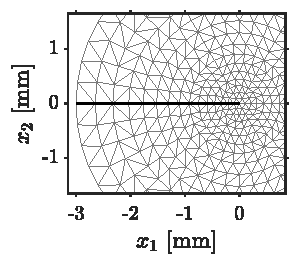
\includegraphics[width=\linewidth]{figures/mesh_levels/tip_mesh_H2.pdf}
    \caption{$4h_0$}
    \label{fig:mesh-level-H2}
  \end{subfigure}
  \hfill
  \begin{subfigure}[t]{0.315\linewidth}
    \centering
    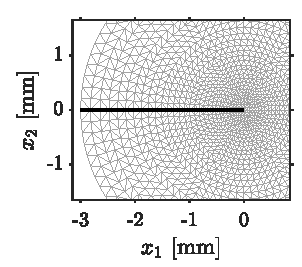
\includegraphics[width=\linewidth]{figures/mesh_levels/tip_mesh_H1.pdf}
    \caption{$2h_0$}
    \label{fig:mesh-level-H1}
  \end{subfigure}
  \hfill
  \begin{subfigure}[t]{0.315\linewidth}
    \centering
    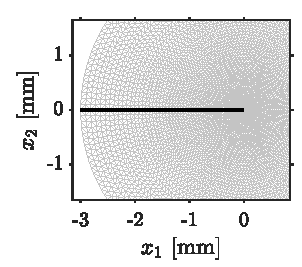
\includegraphics[width=\linewidth]{figures/mesh_levels/tip_mesh_H0.pdf}
    \caption{$h_0$}
    \label{fig:mesh-level-H0}
  \end{subfigure}

  \end{minipage}
  \caption{Structured-tip meshes with a common core radius
  $r_{\mathrm{core}}=3$ mm. The production spacing is
  $h_0=0.027012$ mm; the illustrative $4h_0$ level does not
  satisfy the COD sampling criterion.}
  \label{fig:mesh-levels}
\end{figure}
\FloatBarrier

\subsection{Interaction-integral extraction}
The opening- and sliding-mode SIFs are obtained from the
interaction integral in equivalent-domain form. Let $w$ be its
radial weight function and let $m$ label the opening- or sliding-mode
auxiliary field. The component indices $i,j\in\{1,2\}$ refer
to the current-tip frame and are summed when repeated;
$\delta_{1j}$ is the Kronecker delta. For the actual stress,
strain, and displacement fields
$(\bm\sigma,\bm\varepsilon,\bm u)$, the integral is evaluated over
the material domain $\Omega_k$ defined in Section~\ref{sec:problem}.
The gradient of the radial weight is nonzero only in the interaction
annulus. Here $\dd\Omega$ is the area element,
a comma followed by an index denotes partial differentiation in the
local frame, and the colon denotes tensor contraction. The interaction
integral reads
\begin{equation}
 I^{(m)}=\int_{\Omega_k}
 \left[-(\bm\sigma^{(m)}\!:\bm\varepsilon)\delta_{1j}
 +\sigma_{ij}u^{(m)}_{i,1}
 +\sigma^{(m)}_{ij}u_{i,1}\right]w_{,j}\,\dd\Omega,
 \qquad i,j\in\{1,2\}.\label{eq:interaction}
\end{equation}
The gradients of the actual displacement field are evaluated with
T6 shape functions, whereas the auxiliary stresses are taken from
the asymptotic crack-tip fields. Derivatives of the auxiliary
displacements are evaluated by centered finite differences with
step $h=\max(10^{-7}\ \mathrm m,10^{-5}r)$, where $r$ is the
distance from the current tip. The nodal weight $w$ equals one for
$r\leq r_{\mathrm{in}}$, decreases linearly to zero at
$r_{\mathrm{out}}$, and vanishes beyond the annulus.
Its T6 interpolant provides the gradient used in
Eq.~\eqref{eq:interaction}; numerical integration employs the
16-point triangular rule. For unit auxiliary intensity
$K_{\mathrm{aux}}=1$ in plane strain,
\begin{equation}
 K_m=\frac{E'}{2K_{\mathrm{aux}}}I^{(m)},\qquad
 E'=\frac{E}{1-\nu^2},\qquad m\in\{I,II\}.\label{eq:normalization}
\end{equation}
% TODO: verified interaction-integral and quadrature references.

\subsection{COD-based extraction comparison}
\label{sec:cod-extraction}
Crack-opening displacement (COD) provides a second route to
stress-intensity factors from the same computed elastic field.
Each native crack-face node pair consists of matching upper and
lower T6 nodes on the last segment, with both nodes located at
distance $r$ behind the current tip. The displacement jump
$[\![u_i]\!]$ is the upper-minus-lower difference in component
$u_i$ at such a pair. These existing nodal positions are used
directly; no additional interpolation points are introduced.
The corresponding apparent COD SIFs are
\begin{equation}
 \begin{bmatrix}K_{\mathrm{I}}^{\mathrm{app}}(r)\\K_{\mathrm{II}}^{\mathrm{app}}(r)\end{bmatrix}
 =\frac{\mu}{\kappa+1}\sqrt{\frac{2\pi}{r}}
 \begin{bmatrix}{[\![u_2]\!]}\\{[\![u_1]\!]}\end{bmatrix},
 \qquad \kappa=3-4\nu.\label{eq:cod}
\end{equation}
Here $\kappa$ is the dimensionless plane-strain Kolosov constant.
Linear and quadratic fits of the apparent SIFs against the normalized
distance $r/\Delta a$ are extrapolated to $r=0$. The four fitting
intervals are $[0.04,0.20]$, $[0.04,0.30]$, $[0.08,0.30]$, and
$[0.12,0.30]$. The intervals overlap, so their sampling counts are
not additive. In the stated order, the numbers of native crack-face
node pairs are 19, 28, 23, and 18 for the $2h_0$ mesh;
38, 55, 44, and 34 for the production $h_0$ mesh; and
74, 108, 86, and 67 for the $h_0/2$ mesh.

The prescribed qualification criterion requires at least 12 pairs
in each fitting interval. The illustrative $4h_0$ core provides
10, 15, 12, and 9 pairs, respectively, and fails this criterion
in the first and fourth intervals. It is therefore excluded from
the physical SIF and MTS comparisons. Linear and quadratic fitting
over the four intervals gives eight COD estimates from the same
finite-element displacement field, not eight independent elastic
solutions. Only the EDI SIFs determine subsequent MTS directions,
and the differences among COD fits do not represent a statistical
uncertainty interval.

\subsection{Numerical acceptance and extraction checks}
The assembled stiffness system is reduced to the free degrees of
freedom and symmetrized as specified by the verified formulation.
A symmetric approximate minimum-degree ordering is used together
with symmetric Gauss--Seidel preconditioning and the
preconditioned conjugate-gradient method (PCG). The reported-residual
tolerance is $10^{-10}$, the maximum iteration count is 5000, and
the independently calculated true-relative-residual acceptance
criterion is $5\times10^{-10}$. Prescribed displacement
constraints are enforced exactly.
For the finer fixed-geometry sensitivity meshes only, the PCG iteration
may stagnate at a residual level slightly above the prescribed tolerance
because of finite-precision effects. In that case, one Krylov restart
from the returned iterate is permitted, using the
same matrix, right-hand side, SGS factors, tolerance, and iteration limit.
The final PCG and independently recomputed residual gates are unchanged;
a restart therefore resets the recurrence but does not relax acceptance.
SIF extraction and MTS direction selection are performed
only on fields satisfying these residual criteria.

As a separate test of the extraction procedure, nodal
displacements are prescribed from analytical pure-I, pure-II, and
small mixed-mode asymptotic fields, with
$(K_{\mathrm{I}},K_{\mathrm{II}})=(1,10^{-4})$ in the mixed case.
The allowed recovery and small mixed-mode relative errors are
$2\times10^{-4}$; the limits for pure-mode cross-leakage and
superposition are $10^{-10}$. On the production meshes, the largest
observed small mixed-mode relative error is
$\SyntheticRelativeError$. Because the fields are prescribed rather
than obtained by solving the plate boundary-value problem, these
tests qualify modal extraction and mesh topology but do not bound
the error of the physical stress-intensity factors.

The production path contains accepted physical solutions through
$P_{23}$. The candidate extension to $P_{24}$ passes geometric
and prescribed-field qualification but has no accepted elastic
solution. Across the accepted $P_2$--$P_{23}$ solves, the
largest true relative residual is about $\MaxTrueResidual$,
with 2442--3011 PCG iterations. Figure~\ref{fig:quality}
summarizes these numerical acceptance diagnostics, whose
full-precision values are retained in the saved evidence.

\subsection{Crack-increment refinement family}
The influence of the crack increment is examined using
three independently propagated paths with
\[
 \Delta a\in\{4,2,1\}\ \mathrm{mm}.
\]
These calculations use a common dimensionless coarse family,
distinct from the production 4-mm calculation with exterior law M0
and structured-tip spacing $h_0$. The local tip spacing is twice
the production dimensionless tip spacing, and the exterior follows
the dimensionless M1 sizing law. Thus
\begin{equation}
 \frac{h_{\rm tip}}{\Delta a}
 =2(0.00675308135),\qquad
 \frac{r_{\mathrm{in}}}{\Delta a}=0.10,\qquad
 \frac{r_{\mathrm{out}}}{\Delta a}=0.65,\qquad
 \frac{r_{\mathrm{core}}}{\Delta a}=0.75.
 \label{eq:increment-family}
\end{equation}
The exterior follows the M1 family, with maximum requested
element size $h_{\mathrm{far}}$ and grading transition length
$L_{\mathrm{tr}}$ given by
\[
 \frac{h_{\mathrm{far}}}{\Delta a}=1.25,\qquad
 \frac{L_{\mathrm{tr}}}{\Delta a}=1.00,
\]
and with far-field grading slope 0.15 and boundary-metric
growth 0.35. The absolute structured-tip spacing, core
radius, interaction-domain radii, and exterior scales
therefore decrease with $\Delta a$. This comparison tests a
coupled increment/discretization family; it does not isolate
the crack increment with the physical mesh fixed.

All three calculations retain the accepted Stage-I initiation point
and frozen frame, but use their own first-segment lengths and
independently solved $P_1$ states. Every subsequent vertex is
generated from the corresponding path's own SIF/MTS history
until its accumulated crack length reaches 92 mm.
Corresponding-tip positions and directions are compared at
$a=4,8,\ldots,92$ mm, the exact common lengths of the three
histories; no trajectory interpolation is involved. Separately,
linear interpolation between solved states of each history provides
an estimate of the mode-mixity zero
$q_{\mathrm{K}}=0$ [Eq.~\eqref{eq:mode-mixity}]. This is an
event-location diagnostic, not an independently solved
local-symmetry state.

\subsection{Centered-hole symmetric control}
To assess reflection symmetry and the local angular response of the
numerical procedure, we consider a centered-hole plate with the same
overall dimensions and hole radius. The hole center is
$(0.150,0)$ m, and the crack starts from its rightmost point,
\[
 P_0=(0.180,0)\ \mathrm m,
 \qquad
 P_1=(0.184,0)\ \mathrm m,
\]
with $\Delta a=4$ mm. The straight crack is reflection symmetric
and therefore has a pure mode-I field in the ideal continuum problem.
The one-step angular response is probed by prescribing five
two-segment crack geometries,
\[
 \theta_2\in\{-0.10^\circ,-0.05^\circ,0,
                 +0.05^\circ,+0.10^\circ\},
\]
and solving each geometry independently with the same tip
discretization, EDI extraction, and elastic solver as in the
asymmetric case. Let $F$ denote the predicted direction of the
third segment. The one-step MTS map is
\begin{equation}
 F(\theta_2)=\theta_3
 =\theta_2+
 \alpha_{\mathrm{MTS}}\!\left(K_{\mathrm{I}}(\theta_2),K_{\mathrm{II}}(\theta_2)\right).
 \label{eq:symmetric-map}
\end{equation}

At the straight state,
\[
 K_{\mathrm{I}}(0)=0.42541\ \mathrm{MPa}\sqrt{\mathrm m},
 \qquad
 \frac{K_{\mathrm{II}}(0)}{K_{\mathrm{I}}(0)}=6.22\times10^{-9},
\]
and the predicted next direction is
$F(0)=-7.13\times10^{-7}$ degrees, numerically indistinguishable from the
symmetry line at the scale relevant here. The perturbed probes give the
map summarized in Table~\ref{tab:symmetric-stability}.

\begin{table}[htbp]
\centering
\small
\caption{One-step directional map for the centered-hole symmetric control.
The prescribed second-segment angle and the predicted third-segment direction are shown.}
\label{tab:symmetric-stability}
\begin{tabular*}{0.64\linewidth}{@{\extracolsep{\fill}}rr}
\toprule
$\theta_2$ [deg] & $F(\theta_2)=\theta_3$ [deg]\\
\midrule
$-0.10$ & $+0.011415$\\
$-0.05$ & $+0.005708$\\
$0$     & $-7.13\times10^{-7}$\\
$+0.05$ & $-0.005708$\\
$+0.10$ & $-0.011415$\\
\bottomrule
\end{tabular*}
\end{table}

The opening-mode intensity is approximately even in the
prescribed perturbation $\theta_2$, whereas the signed mode-mixity
ratio and $F(\theta_2)$ exhibit the expected approximately odd
responses under reflection. The small residual at the straight
configuration illustrates that these symmetry relations are
recovered numerically rather than as exact identities.
The two symmetric finite-difference estimates are
\[
 \frac{F(+0.05^\circ)-F(-0.05^\circ)}{0.10^\circ}
 =-0.11416,
 \qquad
 \frac{F(+0.10^\circ)-F(-0.10^\circ)}{0.20^\circ}
 =-0.11415,
\]
and a least-squares fit constrained through the origin yields the local
slope estimate
\begin{equation}
 F'(0)\approx-0.11415.
 \label{eq:symmetric-multiplier}
\end{equation}
For these two-segment geometries at $\Delta a=4$ mm,
the next-segment angular response changes sign and is
approximately 8.8 times smaller than the imposed perturbation.
Because later steps change the complete crack geometry,
they cannot be interpreted as repeated applications of
the same scalar map $F$. The fitted slope therefore
characterizes the local one-step response, not stability
of the evolving trajectory.

\section{Crack-trajectory results}
\label{sec:results}
\subsection{Accepted path and direction history}
The prescribed radial segment $P_0P_1$ establishes the first
crack-tip configuration. Under the unit reference traction, its
opening- and sliding-mode SIFs are
$K_{\mathrm{I}}^{(1)}=0.36648$ and
$K_{\mathrm{II}}^{(1)}=4.1983\times10^{-6}$ MPa$\sqrt{\mathrm m}$,
respectively. Their small positive mode-mixity ratio gives an
initial clockwise correction,
$\Delta\theta_2=\theta_2=-0.0013127^\circ$.
Each subsequent accepted crack direction is obtained from a newly
solved elastic field, producing the history through $P_{23}$.

Figure~\ref{fig:trajectory} shows the resulting $P_0$--$P_{23}$
polyline, with a solid line reserved for accepted crack geometry.
The total accepted length is 92 mm. Its last tip and remaining
horizontal clearance from the right boundary are
\begin{equation}
 P_{23}=(\LastXMM,\LastYMM)\ \mathrm{mm},\qquad
 2A-x_{23}=\LastLigamentMM\ \mathrm{mm}.
\end{equation}
The next candidate segment, $P_{23}P_{24}$, is shown dashed
because its geometry is qualified but the elastic problem at
$P_{24}$ has not been solved to the acceptance criterion.

The polygonal path initially turns clockwise with increasing
magnitude of its negative inclination. Its segment direction reaches
$\theta_{22}=\MinimumTheta^\circ$ and becomes less negative at
$P_{23}$ (Fig.~\ref{fig:intensities}). This change reflects a
positive incremental turn, not a reversal of vertical motion:
the final accepted segment still points below the horizontal.
The trajectory is piecewise linear, and no continuously curved
path has been solved independently.

% Figure environment maintained inline in main.tex; graphics remain separate PDFs.
\begin{figure}[tbp]
  \centering
  \begin{minipage}{0.8\textwidth}
  \centering
  \begin{subfigure}[t]{0.94\linewidth}
    \centering
    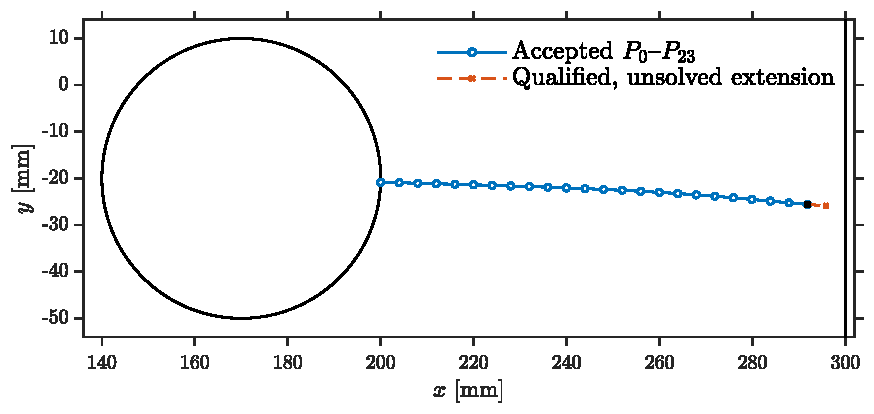
\includegraphics[width=\linewidth]{figures/trajectory/overview.pdf}
    \caption{Accepted trajectory and proposed extension.}
    \label{fig:trajectory-overview}
  \end{subfigure}

  \medskip

  \begin{subfigure}[t]{0.94\linewidth}
    \centering
    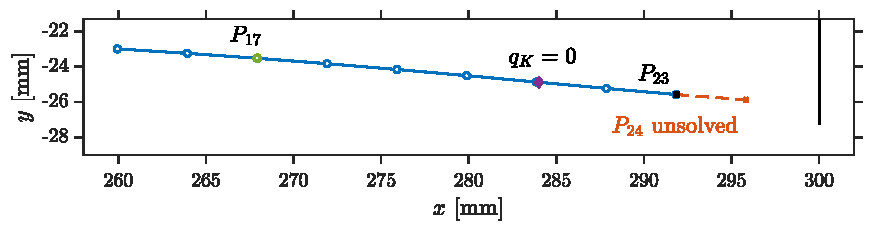
\includegraphics[width=\linewidth]{figures/trajectory/late_detail.pdf}
    \caption{Late-path detail and characteristic locations.}
    \label{fig:trajectory-late}
  \end{subfigure}

  \end{minipage}
  \caption{Crack trajectory from the asymmetric hole.
  Each panel has equal horizontal and vertical scales. The solid line ends at the
  last accepted tip $P_{23}$; the dashed $P_{23}P_{24}$ extension
  has no accepted elastic solution. The diamond marks the
  interpolated mode-mixity zero, not a solved crack tip.}
  \label{fig:trajectory}
\end{figure}


\subsection{Evolution of stress-intensity factors and mode mixity}
The opening-mode intensity increases monotonically along the
accepted 4-mm history, from $K_{\mathrm{I}}=0.36648$ at
$P_1$ to $1.2444$ at $P_{23}$
(Fig.~\ref{fig:intensities}). These values are evaluated under
the same unit remote traction, so the increase reflects the
changing elastic geometry rather than an applied-load history.

The sliding-mode intensity begins close to zero and reaches its
largest positive value, $K_{\mathrm{II}}=0.0025484$,
at $P_{17}$ ($a=68$ mm). The signed mode-mixity ratio
defined in Eq.~\eqref{eq:mode-mixity} attains its positive
maximum, $q_{\mathrm{K}}=0.0032389$, at the same state.
This is a positive maximum, not a maximum of
$|K_{\mathrm{II}}|$: the negative sliding-mode magnitude at
the last accepted tip is larger. After $P_{17}$,
$K_{\mathrm{II}}$ decreases while $K_{\mathrm{I}}$ continues
to rise. The resulting decrease in positive mode mixity
reduces the magnitude of the clockwise MTS turn through
$P_{21}$ (Fig.~\ref{fig:late}).

% Figure environment maintained inline in main.tex; graphics remain separate PDFs.
\begin{figure}[tbp]
  \centering
  \begin{minipage}{0.8\textwidth}
  \centering
  \begin{subfigure}[t]{0.315\linewidth}
    \centering
    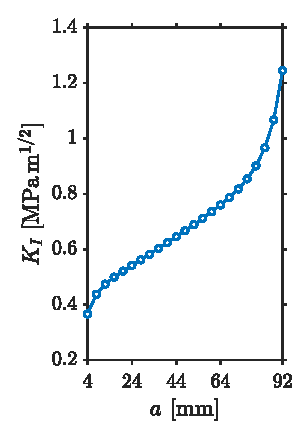
\includegraphics[width=\linewidth]{figures/intensities/KI.pdf}
    \caption{Opening-mode factor $K_{\mathrm{I}}$.}
    \label{fig:intensities-KI}
  \end{subfigure}\hfill
  \begin{subfigure}[t]{0.315\linewidth}
    \centering
    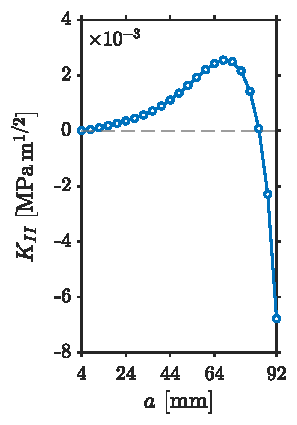
\includegraphics[width=\linewidth]{figures/intensities/KII.pdf}
    \caption{Sliding-mode factor $K_{\mathrm{II}}$.}
    \label{fig:intensities-KII}
  \end{subfigure}\hfill
  \begin{subfigure}[t]{0.315\linewidth}
    \centering
    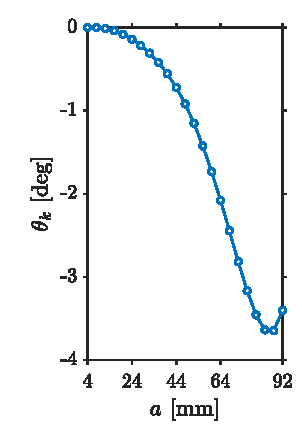
\includegraphics[width=\linewidth]{figures/intensities/theta.pdf}
    \caption{Absolute direction $\theta_k$.}
    \label{fig:intensities-theta}
  \end{subfigure}

  \end{minipage}
  \caption{Opening- and sliding-mode SIFs (MPa$\sqrt{\mathrm m}$)
  and segment direction (degrees) versus accumulated crack length
  $a$ (mm), under unit remote traction. The segment direction
  reaches its minimum at $P_{22}$ and becomes less negative at $P_{23}$.}
  \label{fig:intensities}
\end{figure}


\subsection{Mode-mixity sign change and turning reversal}
The mode-mixity ratio remains positive at
$P_{21}$ ($a=84$ mm), where
$q_{\mathrm{K}}^{(21)}=+8.134267\times10^{-5}$,
but is negative at $P_{22}$ ($a=88$ mm), where
$q_{\mathrm{K}}^{(22)}=-0.0021416$. Thus the
sign reversal is established between two independently solved
accepted states, although neither has zero mode mixity.
For the graphical marker in Figs.~\ref{fig:trajectory-late}
and \ref{fig:late}, linear interpolation between their
values gives
\begin{equation}
 a_{\mathrm{LS}}=a_{21}
 -\frac{\qmix^{(21)}}{\qmix^{(22)}-\qmix^{(21)}}(a_{22}-a_{21})
 \simeq\LSLengthMM\ \mathrm{mm}.\label{eq:zeroestimate}
\end{equation}
Here $a_{\mathrm{LS}}$ denotes only an interpolated estimate of
the crack length at which local symmetry
($K_{\mathrm{II}}=0$) would occur. It is not a solved
zero-mode-II state, and the interpolation does not establish
the physical location with sub-increment accuracy.

The sign change has an immediate directional consequence.
At $P_{21}$ the MTS turn toward $P_{22}$ is still
clockwise, whereas the negative mode mixity at $P_{22}$
produces a counterclockwise turn toward the accepted
$P_{23}$ segment (Fig.~\ref{fig:late}). At that
last solved state, $K_{\mathrm{I}}=1.2444$,
$K_{\mathrm{II}}=-0.0067803$, and
$q_{\mathrm{K}}=-0.0054488$; the MTS rule then
predicts $\Delta\theta_{24}=0.62435^\circ$
and $\theta_{24}=-2.7762^\circ$.
This final prediction specifies the qualified extension,
not an accepted elastic solution at $P_{24}$.

\begin{table}[htbp]\centering\small\setlength{\tabcolsep}{3.5pt}
\caption{Characteristic accepted states. SIFs have units MPa$\sqrt{\mathrm m}$;
angles are in degrees. The interpolated row contains only a graphical
zero estimate, not a solved stress field or crack direction.}
\begin{tabular}{lrrrrrr}\toprule
State & $a$ [mm] & $K_{\mathrm{I}}$ & $K_{\mathrm{II}}$ & $K_{\mathrm{II}}/K_{\mathrm{I}}$ & $\theta_k$ & $\Delta\theta_{k+1}$\\\midrule
\CharacteristicRows
Interpolated & \LSLengthMM & --- & --- & $0$ & --- & ---\\
\bottomrule\end{tabular}\label{tab:states}
\end{table}

% Figure environment maintained inline in main.tex; graphics remain separate PDFs.
\begin{figure}[htbp]
  \centering
  \begin{minipage}{0.8\textwidth}
  \centering
  \begin{subfigure}[t]{0.485\linewidth}
    \centering
    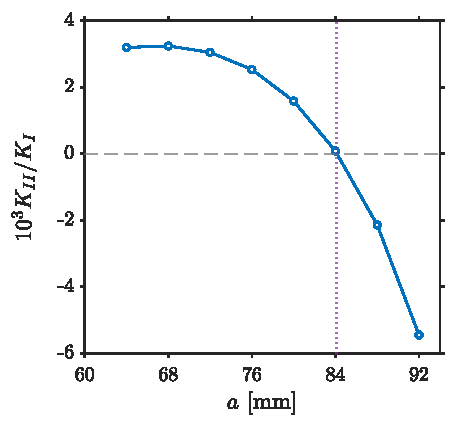
\includegraphics[width=\linewidth]{figures/late/mode_mixity.pdf}
    \caption{Late mode-mixity history.}
    \label{fig:late-mixity}
  \end{subfigure}\hfill
  \begin{subfigure}[t]{0.485\linewidth}
    \centering
    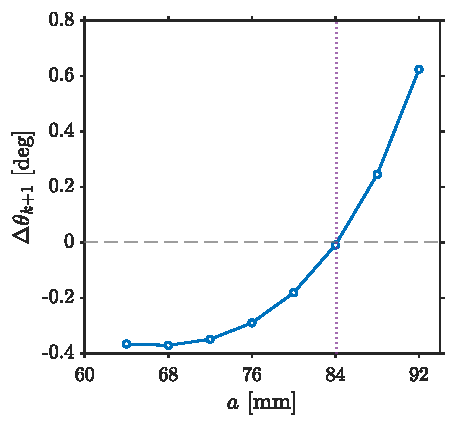
\includegraphics[width=\linewidth]{figures/late/turn.pdf}
    \caption{Incremental MTS turn.}
    \label{fig:late-turn}
  \end{subfigure}

  \end{minipage}
  \caption{Mode-mixity sign change and reversal of the MTS turn.
  The dotted line denotes the interpolated mode-mixity zero.
  The turn computed at $P_{23}$ ($a=92$ mm) predicts the
  proposed, physically unsolved next segment.}
  \label{fig:late}
\end{figure}
\FloatBarrier


\subsection{COD comparison and extraction sensitivity}
Because the sign reversal of mode mixity changes the MTS turning
direction, its persistence under another SIF extraction procedure
is particularly relevant. Each of the eight COD fits gives
$q_{\mathrm{K}}>0$ at $P_{21}$ and $q_{\mathrm{K}}<0$
at $P_{22}$, in agreement with the EDI sign-change bracket.
The quantitative differences depend on the chosen fitting
window and polynomial degree (Fig.~\ref{fig:cod}).
Across 176 fits, the greatest absolute difference between
the COD- and EDI-based MTS turns is
$\MaxCODError^\circ$, at $P_{23}$ for the
linear fit over $[0.12,0.30]\Delta a$.
The quadratic COD turns at that state range from
$\CODQuadMin^\circ$ to $\CODQuadMax^\circ$,
compared with the EDI prediction of $0.62435^\circ$.

The distinction between the sign and magnitude of a small
mode-mixity ratio is important close to local symmetry.
At $P_{21}$, the rear-window linear fit exceeds the
EDI ratio by $\CODNearZeroPercent$\%, although the
corresponding turning-angle difference is only
$\CODNearZeroTurnDiff^\circ$. The relative discrepancy
is consequently sensitive to the small denominator in
the comparison. The two extraction methods thus agree on the sign-change
bracket, although their common displacement solution
precludes an independent estimate of the finite-element
error. The differences among COD fits measure sensitivity
to the extrapolation procedure, not statistical uncertainty.

% Figure environment maintained inline in main.tex; graphics remain separate PDFs.
\begin{figure}[htbp]
  \centering
  \begin{minipage}{0.8\textwidth}
  \centering
  \begin{subfigure}[t]{0.485\linewidth}
    \centering
    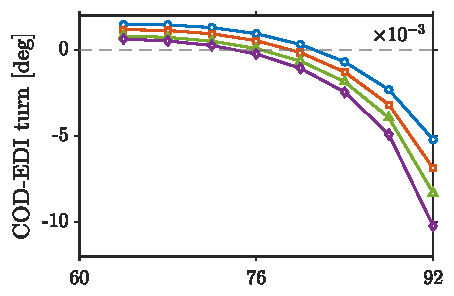
\includegraphics[width=\linewidth]{figures/cod/turn_linear.pdf}
    \caption{Turning-angle differences for linear COD fits.}
    \label{fig:cod-turn-linear}
  \end{subfigure}
  \hfill
  \begin{subfigure}[t]{0.485\linewidth}
    \centering
    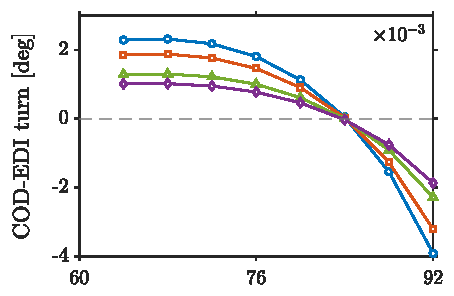
\includegraphics[width=\linewidth]{figures/cod/turn_quadratic.pdf}
    \caption{Turning-angle differences for quadratic COD fits.}
    \label{fig:cod-turn-quadratic}
  \end{subfigure}

  \medskip

  \begin{subfigure}[t]{0.485\linewidth}
    \centering
    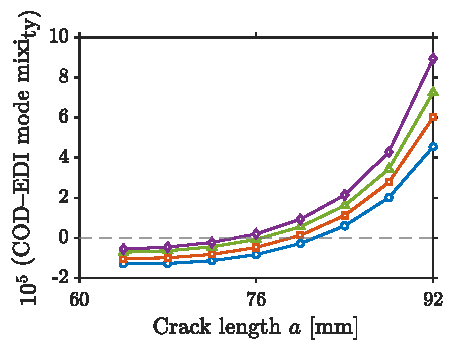
\includegraphics[width=\linewidth]{figures/cod/mixity_linear.pdf}
    \caption{Mode-mixity differences for linear COD fits.}
    \label{fig:cod-mixity-linear}
  \end{subfigure}
  \hfill
  \begin{subfigure}[t]{0.485\linewidth}
    \centering
    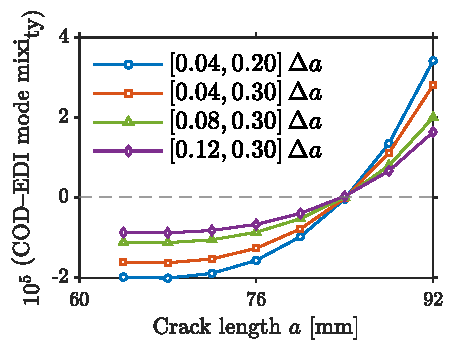
\includegraphics[width=\linewidth]{figures/cod/mixity_quadratic.pdf}
    \caption{Mode-mixity differences for quadratic COD fits.}
    \label{fig:cod-mixity-quadratic}
  \end{subfigure}

  \end{minipage}
  \caption{COD--EDI differences along the late crack path for
  four normalized COD fitting windows and linear or quadratic
  extrapolation. Upper panels compare MTS turns; lower panels
  compare mode-mixity ratios. Zero denotes agreement of the
  extraction methods, not a known exact solution.}
  \label{fig:cod}
\end{figure}
\FloatBarrier


\subsection{Sensitivity to structured-tip resolution}
For comparisons at matched crack lengths, $\delta x$ and $\delta y$ denote
coordinate differences between the compared and baseline paths,
$\delta r=(\delta x^2+\delta y^2)^{1/2}$ is their separation, and
$\delta\theta$ is the difference of absolute directions in the frozen
frame. The symbol $\Delta\theta_{k+1}$ remains reserved for a local MTS
turn. Differences in mode mixity and interpolated crossing length are
denoted by $\delta q_{\mathrm{K}}$ and $\delta a_{\mathrm{LS}}$, respectively.

Two aspects of the characteristic mode-mixity history are
examined on fixed accepted crack geometries. At the positive
maximum $P_{17}$, reducing the structured-tip spacing from
$0.027012$ to $0.013506$ mm changes $K_{\mathrm{I}}$
by $0.00134\%$, $q_{\mathrm{K}}$ by
$1.05\times10^{-6}$, and the MTS turn by
$-1.20\times10^{-4}$ degrees. The small differences arise
from alternative discretizations of the same physical geometry.

The late sign-change bracket provides a more sensitive test.
Table~\ref{tab:tipmesh} compares the $P_{21}$ and
$P_{22}$ fields at three near-tip resolutions spanning
a factor of four in $h_{\mathrm{tip}}$.
For every tested level, $q_{\mathrm{K}}$ remains positive
at $P_{21}$ and negative at $P_{22}$. The bracket
and the corresponding change in MTS turning sense thus persist
under the tested near-tip refinement.

\begin{table}[htbp]
\centering
\small
\setlength{\tabcolsep}{2.6pt}
\caption{Structured-tip sensitivity at fixed $P_{21}$ and $P_{22}$
geometries, with common interaction-domain radii and requested
exterior sizing. The reported $a_{\mathrm{LS}}$ values are
interpolated sign-change estimates, not independently solved
zero-mode-II states.}
\label{tab:tipmesh}
\begin{tabular}{lrrrrrr}
\toprule
Resolution & $h_{\rm tip}$ [mm] &
$q_{\mathrm{K}}(P_{21})$ & $\Delta\theta_{22}$ [deg] &
$q_{\mathrm{K}}(P_{22})$ & $\Delta\theta_{23}$ [deg] &
$a_{\rm LS}$ [mm]\\
\midrule
$2h_0$ & 0.054025 & $+7.7957\times10^{-5}$ & $-0.008933$ &
$-2.1451\times10^{-3}$ & $+0.245805$ & 84.14027\\
$h_0$ & 0.027012 & $+8.1343\times10^{-5}$ & $-0.009321$ &
$-2.1416\times10^{-3}$ & $+0.245406$ & 84.14637\\
$h_0/2$ & 0.013506 & $+8.3031\times10^{-5}$ & $-0.009515$ &
$-2.1399\times10^{-3}$ & $+0.245207$ & 84.14941\\
\bottomrule
\end{tabular}
\end{table}

The linearly interpolated estimate $a_{\mathrm{LS}}$
varies from $84.14027$ mm at $2h_0$ through
$84.14637$ mm at $h_0$ to $84.14941$ mm at
$h_0/2$. Its successive shifts of $6.10$ and
$3.04~\mu\mathrm{m}$ give an indicative contraction
ratio corresponding to an apparent order of approximately
$1.00$. This figure describes the mesh sensitivity of an
\emph{interpolated estimate}, not convergence of a solved
zero-mode-II point. Because the contributing physical states
are separated by a 4-mm crack increment, the small shifts
cannot be interpreted as micrometer-scale accuracy of the
local-symmetry location.

Propagation with the $2h_0$ tip mesh produces a path nearly
indistinguishable from the $h_0$ trajectory at specimen scale
[Fig.~\ref{fig:tipres-trajectory}]. The maximum vertical-coordinate
difference is
$0.12760~\mu\mathrm{m}$ and the maximum Euclidean separation of
corresponding tips is $0.12800~\mu\mathrm{m}$, both at $P_{23}$. The
maximum absolute direction difference is $0.24539$ millidegrees at
$P_{22}$ [Figs.~\ref{fig:tipres-dy} and \ref{fig:tipres-dtheta}].

% Figure environment maintained inline in main.tex; graphics remain separate PDFs.
\begin{figure}[!t]
  \centering
  \captionsetup[subfigure]{justification=raggedright,singlelinecheck=false}
  \begin{minipage}{0.8\textwidth}
  \centering

  \begin{subfigure}[t]{0.94\linewidth}
    \centering
    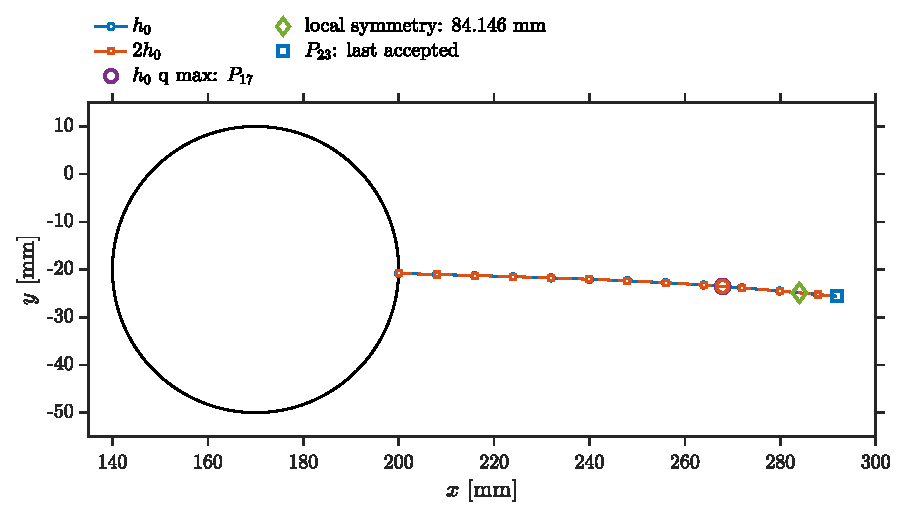
\includegraphics[width=\linewidth]{figures/tip_resolution_sensitivity/trajectory.pdf}
    \caption{Trajectories with structured-tip spacings $h_0$ and $2h_0$.}
    \label{fig:tipres-trajectory}
  \end{subfigure}

  \par\smallskip

  \begin{subfigure}[t]{0.315\linewidth}
    \centering
    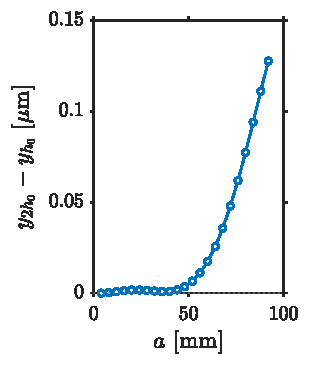
\includegraphics[width=\linewidth]{figures/tip_resolution_sensitivity/vertical_deviation.pdf}
    \caption{Vertical tip-coordinate difference, $y_{2h_0}-y_{h_0}$.}
    \label{fig:tipres-dy}
  \end{subfigure}
  \hfill
  \begin{subfigure}[t]{0.315\linewidth}
    \centering
    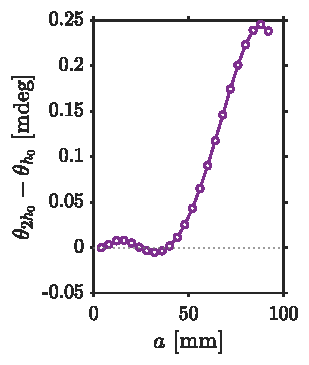
\includegraphics[width=\linewidth]{figures/tip_resolution_sensitivity/direction_deviation.pdf}
    \caption{Crack-direction difference, $\theta_{2h_0}-\theta_{h_0}$.}
    \label{fig:tipres-dtheta}
  \end{subfigure}
  \hfill
  \begin{subfigure}[t]{0.315\linewidth}
    \centering
    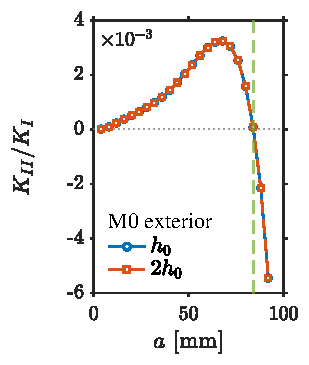
\includegraphics[width=\linewidth]{figures/tip_resolution_sensitivity/mode_mixity.pdf}
    \caption{Mode-mixity histories for the two tip resolutions.}
    \label{fig:tipres-q}
  \end{subfigure}

  \end{minipage}
  \caption{Effect of structured-tip resolution on the propagated
  trajectory. The $h_0$ and $2h_0$ paths share the interaction-domain
  radii and the M0 exterior sizing law. Panel (d) shows
  $K_{\mathrm{II}}/K_{\mathrm{I}}$. The diamond indicates the
  interpolated mode-mixity zero of the $h_0$ path.}
  \label{fig:tip-resolution-sensitivity}
\end{figure}

The two independently generated paths also retain the
positive mode-mixity maximum at $P_{17}$ and the sign-change
bracket between $P_{21}$ and $P_{22}$
[Fig.~\ref{fig:tipres-q}]. The largest difference
in $q_{\mathrm{K}}$ is $2.65\times10^{-7}$.
Linear interpolation of the two independently propagated
$P_{21}$--$P_{22}$ brackets gives
$a_{\mathrm{LS}}=84.14637$ mm for $h_0$ and
$84.146276$ mm for $2h_0$, a difference of
$-0.000094$ mm ($-0.094~\mu\mathrm{m}$). As above, this is only a
sub-increment sensitivity diagnostic, not a micrometer-accurate physical
location of local symmetry.

The positive mode-mixity maximum, sign-change bracket, and
turning reversal persist across the tested structured-tip
resolutions, both on fixed geometries and along the propagated
$2h_0$ trajectory. This evidence concerns the stated
mesh perturbations; the conforming exterior connectivity
also changes when the core is remeshed.

% Keep the short exterior-mesh discussion together beside its figures.
\Needspace{25\baselineskip}
\subsection{Sensitivity to exterior-mesh density}
Coarsening the exterior mesh has little effect on the SIFs
of the fixed $P_{17}$ and $P_{22}$ geometries. We therefore
examined its influence on the complete trajectory by propagating
the M1 discretization from the common first segment $P_0P_1$.
All later crack directions follow from the M1 solutions
rather than from the M0 path.

The two trajectories are nearly coincident at the specimen scale
[Fig.~\ref{fig:m1mesh-trajectory}]. Their small separation becomes
apparent in the coordinate and angular differences in
Fig.~\ref{fig:m1-mesh-sensitivity}. The maximum vertical-coordinate
difference is $0.06734~\mu\mathrm{m}$, the maximum Euclidean separation of
corresponding tips is $0.06742~\mu\mathrm{m}$, and the maximum absolute direction
difference is $0.07304$ millidegrees, or $7.30\times10^{-5}$ degrees
[Figs.~\ref{fig:m1mesh-dy} and \ref{fig:m1mesh-dtheta}].

The event sequence is also preserved when the exterior
mesh is coarsened. Both propagated trajectories attain
their positive mode-mixity maximum at $P_{17}$
($a=68$ mm), with a positive ratio at $P_{21}$ and
a negative ratio at $P_{22}$ [Fig.~\ref{fig:m1mesh-q}].
Their largest absolute difference in $q_{\mathrm{K}}$
is $2.89\times10^{-7}$. Linear interpolation of
the respective $P_{21}$--$P_{22}$ brackets gives
$a_{\mathrm{LS}}=84.14637$ mm for M0 and
$84.146$ mm for M1, a difference of $0.000322$ mm
($0.322~\mu\mathrm{m}$). This sub-increment difference is reported only as a
sensitivity diagnostic; neither interpolated value has physical precision
at the micrometer scale.

\begin{samepage}
The characteristic event sequence remains unchanged
under the tested coarsening of the \emph{exterior} mesh.
Because the near-tip discretization and interaction-domain
radii are unchanged, the comparison does not establish
general mesh independence.
\end{samepage}

% Figure environment maintained inline in main.tex; graphics remain separate PDFs.
\begin{figure}[htbp]
  \centering
  \captionsetup[subfigure]{justification=raggedright,singlelinecheck=false}
  \begin{minipage}{0.8\textwidth}
  \centering

  \begin{subfigure}[t]{0.94\linewidth}
    \centering
    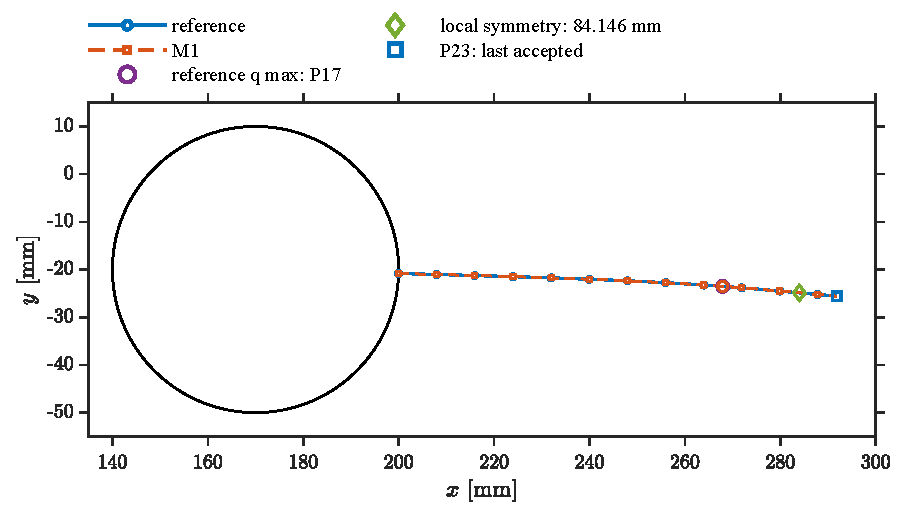
\includegraphics[width=\linewidth]{figures/m1_mesh_sensitivity/trajectory.pdf}
    \caption{Crack trajectories with the M0 and M1 exterior sizing laws.}
    \label{fig:m1mesh-trajectory}
  \end{subfigure}

  \par\smallskip

  \begin{subfigure}[t]{0.315\linewidth}
    \centering
    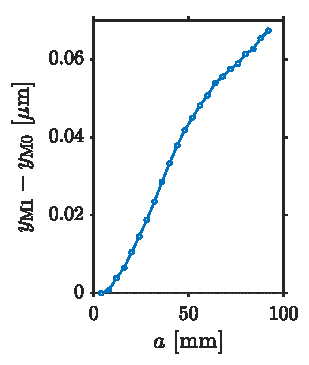
\includegraphics[width=\linewidth]{figures/m1_mesh_sensitivity/vertical_deviation.pdf}
    \caption{Vertical tip-coordinate difference, $y_{\mathrm{M1}}-y_{\mathrm{M0}}$.}
    \label{fig:m1mesh-dy}
  \end{subfigure}
  \hfill
  \begin{subfigure}[t]{0.315\linewidth}
    \centering
    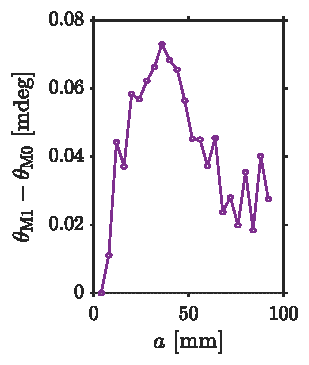
\includegraphics[width=\linewidth]{figures/m1_mesh_sensitivity/direction_deviation.pdf}
    \caption{Crack-direction difference, $\theta_{\mathrm{M1}}-\theta_{\mathrm{M0}}$.}
    \label{fig:m1mesh-dtheta}
  \end{subfigure}
  \hfill
  \begin{subfigure}[t]{0.315\linewidth}
    \centering
    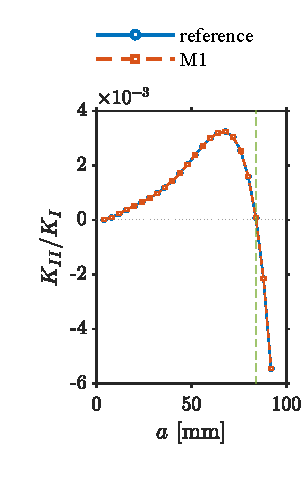
\includegraphics[width=\linewidth]{figures/m1_mesh_sensitivity/mode_mixity.pdf}
    \caption{Mode-mixity histories for M0 and M1.}
    \label{fig:m1mesh-q}
  \end{subfigure}

  \end{minipage}
  \caption{Effect of exterior-mesh coarsening on the crack path.
  The M0 and M1 trajectories are propagated separately with
  identical near-tip discretizations and interaction-domain radii.
  Panel (d) shows $K_{\mathrm{II}}/K_{\mathrm{I}}$. The diamond marks
  the interpolated mode-mixity zero of the
  M0 path.}
  \label{fig:m1-mesh-sensitivity}
\end{figure}
\FloatBarrier

\subsection{Coupled crack-increment and discretization refinement}
The paths computed with $\Delta a=4$, 2, and 1 mm remain
nearly coincident through 92 mm of growth
[Fig.~\ref{fig:inc-trajectory}]. Their differences in
tip position and segment direction nevertheless decrease with
refinement [Fig.~\ref{fig:increment-sensitivity}].
In this study, the near-tip mesh, interaction domain, and
exterior scales are reduced together with $\Delta a$,
as specified in Section~\ref{sec:numerics}; hence the comparison
concerns a coupled increment/discretization family.

% Figure environment maintained inline in main.tex; graphics remain separate PDFs.
\begin{figure}[htbp]
  \centering
  \captionsetup[subfigure]{justification=raggedright,singlelinecheck=false}
  \begin{minipage}{0.8\textwidth}
  \centering

  \begin{subfigure}[t]{0.94\linewidth}
    \centering
    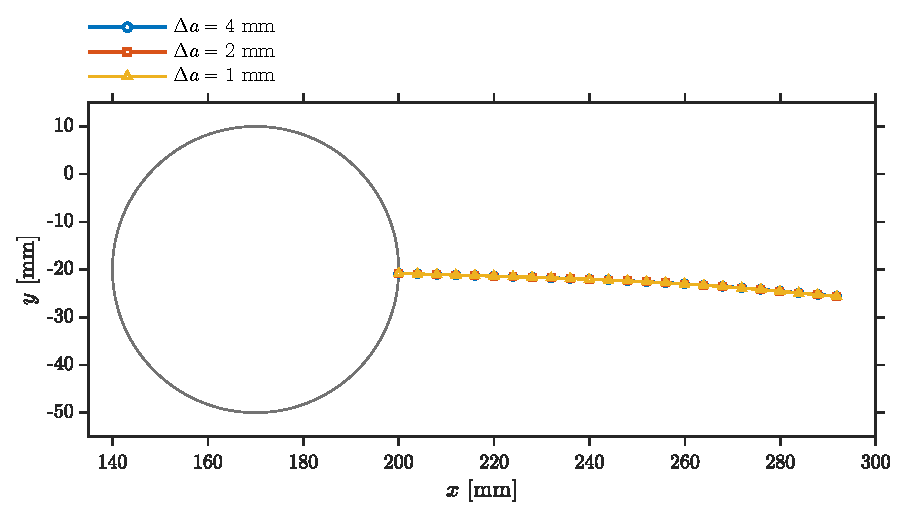
\includegraphics[width=\linewidth]{figures/increment_sensitivity/trajectory.pdf}
    \caption{Independently propagated crack trajectories for
    $\Delta a=4$, 2, and 1 mm, all continued to 92 mm.}
    \label{fig:inc-trajectory}
  \end{subfigure}
  \par\smallskip
  \begin{subfigure}[t]{0.315\linewidth}
    \centering
    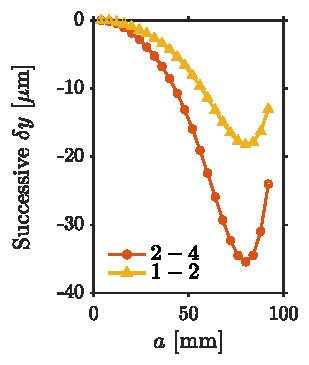
\includegraphics[width=\linewidth]{figures/increment_sensitivity/vertical_deviation.pdf}
    \caption{Successive vertical tip-coordinate differences.}
    \label{fig:inc-dy}
  \end{subfigure}
  \hfill
  \begin{subfigure}[t]{0.315\linewidth}
    \centering
    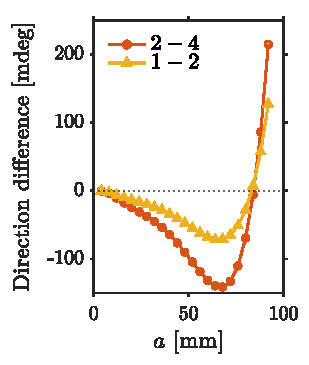
\includegraphics[width=\linewidth]{figures/increment_sensitivity/direction_deviation.pdf}
    \caption{Successive crack-direction differences.}
    \label{fig:inc-dtheta}
  \end{subfigure}
  \hfill
  \begin{subfigure}[t]{0.315\linewidth}
    \centering
    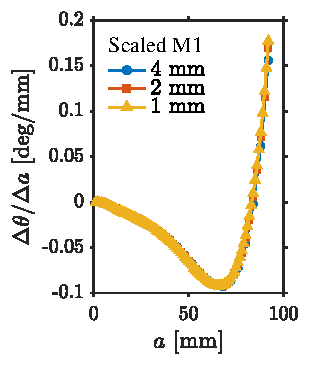
\includegraphics[width=\linewidth]{figures/increment_sensitivity/turn_density.pdf}
    \caption{Turning density along the three trajectories.}
    \label{fig:inc-turn-density}
  \end{subfigure}

  \end{minipage}
  \par\medskip
  \caption{Coupled crack-increment and discretization refinement.
  The $4$-, $2$-, and $1$-mm paths share dimensionless mesh and
  interaction-domain scales within the scaled-M1 family.
  Panel (b) shows $y_{2\,\mathrm{mm}}-y_{4\,\mathrm{mm}}$ and
  $y_{1\,\mathrm{mm}}-y_{2\,\mathrm{mm}}$ at exact common crack lengths.
  Panel (c) shows the corresponding differences of absolute directions
  in the frozen initiation frame. Panel (d) shows
  turning density $\Delta\theta/\Delta a$ on each path's native grid.}
  \label{fig:increment-sensitivity}
\end{figure}
\FloatBarrier

Table~\ref{tab:increment-pairwise} compares tip positions
and directions at crack lengths common to all three paths.
The maximum tip separation contracts from
$35.472~\mu\mathrm{m}$ for 4 versus 2 mm to
$18.291~\mu\mathrm{m}$ for 2 versus 1 mm.
The corresponding vertical differences decrease from
$35.418$ to $18.263~\mu\mathrm{m}$, while the
maximum absolute direction difference decreases from
$214.931$ to $127.391$ millidegrees.

\begin{table}[htbp]
\centering
\small
\setlength{\tabcolsep}{4.0pt}
\caption{Successive differences between independently propagated paths in
the dimensionless crack-increment refinement family. Comparisons use exact
common crack lengths; no path interpolation is used.}
\label{tab:increment-pairwise}
\begin{tabular}{lrrrr}
\toprule
Comparison &
$\max|\delta y|$ [$\mu$m] &
$\max\delta r$ [$\mu$m] &
$\max|\delta\theta|$ [mdeg] &
$\max|\delta q_{\mathrm{K}}|$\\
\midrule
2 mm $-$ 4 mm & 35.4181 & 35.4721 & 214.931 & $2.48578\times10^{-3}$\\
1 mm $-$ 2 mm & 18.2629 & 18.2911 & 127.391 & $1.41618\times10^{-3}$\\
\bottomrule
\end{tabular}
\end{table}

The contraction ratios are 1.939 for maximum tip
separation and 1.687 for maximum direction difference.
If $d$ denotes a successive-difference maximum,
the descriptive quantity
$p=\log_2(d_{\Delta a}/d_{\Delta a/2})$
takes values of approximately 0.96 and 0.75,
respectively. These are not formal Richardson orders:
the compared paths result from recursively updated
geometries, the maximizers need not occur at the same
crack length, and both the increment and discretization
scales change. These values describe contraction within the three-level family
and cannot be regarded as measured asymptotic rates.

The normalized mode-mixity response exhibits a
complementary trend. As shown in
Table~\ref{tab:increment-characteristic}, the
positive maximum of $q_{\mathrm{K}}$ falls from
$3.23937\times10^{-3}$ at 4 mm to
$1.61266\times10^{-3}$ at 2 mm and
$8.04068\times10^{-4}$ at 1 mm.
Despite this nearly proportional decrease, the
maximum divided by $\Delta a$ changes by only
about $0.71\%$ between the coarsest and finest levels.
The corresponding MTS turning density ranges from
$-0.092799$ to $-0.092139$ deg/mm.
The turning-density histories in
Fig.~\ref{fig:inc-turn-density} exhibit similar shapes
on their respective crack-length grids, although this
does not establish convergence of a smooth limiting
curvature.

\begin{table}[tbp]
\centering
\small
\setlength{\tabcolsep}{3.6pt}
\caption{Characteristic quantities in the crack-increment refinement
family. The local-symmetry location is obtained by linear interpolation
between the two solved states bracketing $q_{\mathrm{K}}=0$.}
\label{tab:increment-characteristic}
\begin{tabular}{rrrrrr}
\toprule
$\Delta a$ [mm] &
$a(q_{\mathrm{K},\max})$ [mm] &
$q_{\mathrm{K},\max}$ &
\shortstack[c]{$q_{\mathrm{K},\max}/\Delta a$\\{}[mm$^{-1}$]} &
\shortstack[c]{$(\Delta\theta/\Delta a)_{q_{\max}}$\\{}[deg/mm]} &
$a_{\rm LS}$ [mm]\\
\midrule
4 & 68 & $3.2394\times10^{-3}$ & $8.0984\times10^{-4}$ &
$-0.092799$ & 84.148913\\
2 & 66 & $1.6127\times10^{-3}$ & $8.0633\times10^{-4}$ &
$-0.092398$ & 83.550120\\
1 & 66 & $8.0407\times10^{-4}$ & $8.0407\times10^{-4}$ &
$-0.092139$ & 83.268112\\
\bottomrule
\end{tabular}
\end{table}

The positive maximum is sampled at $a=68$ mm on the 4-mm path and
at $a=66$ mm on the two finer paths; the values therefore do not
correspond to an identical crack length. Nevertheless, their
near-proportional decrease with $\Delta a$, together with the
stability of turning density, is consistent with the conditional
curvature--MTS correspondence in Eq.~\eqref{eq:curvature-mts}.
The observed behavior may be summarized as
\begin{equation}
 q_{\mathrm{K}}=O(\Delta a),\qquad
 \Delta\theta=O(\Delta a),
 \label{eq:increment-scaling}
\end{equation}
within the investigated numerical family. Three coupled refinement
levels provide evidence of this scaling rather than an
independent proof of asymptotic convergence.

The estimated position of the mode-mixity sign change
also shifts less with successive refinement. Linear
interpolation gives $a_{\mathrm{LS}}=84.148913$,
$83.550120$, and $83.268112$ mm for the three
levels. The successive differences are $0.59879$
and $0.28201$ mm, giving a contraction ratio of
2.12 and a descriptive apparent order near 1.09.
On the 1-mm path, the sign change is bracketed by
the solved states at 83 and 84 mm. None of these
interpolated estimates is itself a solved
zero-$K_{\mathrm{II}}$ state.

\begin{samepage}
The nearly proportional decrease of the raw mode-mixity
maxima and the stability of the increment-normalized
measures accord with the conditional MTS--curvature
relation in Eq.~\eqref{eq:curvature-mts}. The available
three-level evidence does not establish a unique smooth
limiting trajectory.
\end{samepage}

\Needspace{14\baselineskip}
\section{Discussion}
\label{sec:discussion}
\subsection{Mechanical interpretation of the turning reversal}
The turning sense of each new segment follows from the current-tip
mode-mixity ratio through the MTS criterion. Positive
$q_{\mathrm{K}}$ produces a clockwise correction under the adopted
sign convention; when $q_{\mathrm{K}}$ becomes negative, the correction
is counterclockwise. The positive mode-mixity maximum at $P_{17}$,
followed by the sign change between $P_{21}$ and $P_{22}$, therefore
explains the changes in turning direction along the accepted
trajectory. At the same time, $K_{\mathrm{I}}$ increases under the
fixed unit remote traction. The reversal is consequently a change in
the relative sliding-mode contribution, not a decrease in the
opening-mode intensity or a reversal of the crack's vertical
displacement.

The remaining horizontal ligament is only $\LastLigamentMM$ mm at
$P_{23}$, suggesting that the approaching traction-free right
boundary may contribute to the late mixed-mode response. That
influence cannot, however, be identified separately from the
increasing crack length and the evolving crack geometry in the
present calculations. A controlled comparison at different
boundary distances would be needed to determine its contribution.
The computed SIFs establish the MTS turning mechanism, but not
a unique physical cause for their evolution.

\subsection{Numerical sensitivity and the smooth-path interpretation}
The verification studies address different sources of uncertainty.
Prescribed asymptotic fields test the implementation of SIF
extraction, whereas COD fitting and the interaction integral
provide two estimates derived from the same finite-element
displacement field. Their agreement near the mode-mixity sign
change lends support to the extracted turning sense, but cannot
serve as an independent validation of the underlying elastic
solution. Likewise, the centered-hole test establishes the
expected reflection symmetry and a small one-step angular
response, without implying attraction of an entire evolving
trajectory.

The independently propagated mesh studies examine whether
discretization differences alter the recursive path construction.
Coarsening the exterior mesh in M1 preserves the paired near-tip
core and interaction-domain support; changing the structured-tip
spacing preserves the requested exterior sizing law, though
conforming remeshing can change the exterior connectivity.
Both propagated alternatives retain the positive mode-mixity
maximum and the $P_{21}$--$P_{22}$ sign-change bracket.
Their maximum corresponding-tip separations, $0.0674$ and
$0.128~\mu\mathrm{m}$, respectively, are small relative to
the crack increments. These observations demonstrate low
sensitivity to the two tested mesh perturbations, not
independence of the solution from all discretization choices.

The 4/2/1-mm trajectories probe a different aspect of the
algorithm. In that family, the crack increment, structured-tip
spacing, interaction-domain radii, and exterior mesh scales
decrease together. Successive differences in tip position and
direction contract, while the positive maximum of
$q_{\mathrm{K}}$ decreases approximately in proportion to
$\Delta a$. Its increment-normalized value and the
corresponding turning density remain comparatively stable.
The small-mixity MTS expansion thus provides a plausible
connection to the signed curvature of a smooth limiting
trajectory [Eq.~\eqref{eq:curvature-mts}], provided such a
limit exists and the discrete turning densities converge.
Neither a formal convergence order nor the separate
contribution of crack-increment error follows from these
three coupled refinement levels. This distinction also
limits direct comparison with studies that vary the
increment alone, including the two-level comparison of
Fang et al.~\cite{FangEtAl2020}.

Table~\ref{tab:independent-sensitivity} compares the
exterior-mesh and structured-tip perturbations. The larger
differences observed in the coupled 4/2/1-mm family do
not isolate the contribution of any individual numerical scale.

\begin{table}[htbp]
\centering
\small
\setlength{\tabcolsep}{4.2pt}
\caption{Trajectory sensitivity to exterior-mesh and structured-tip
resolution. Differences in $a_{\mathrm{LS}}$ compare linearly
interpolated mode-mixity zeros between $P_{21}$ and $P_{22}$.}
\label{tab:independent-sensitivity}
\begin{tabular}{lrrrrr}
\toprule
Perturbation &
$\max|\delta y|$ [$\mu$m] &
$\max\delta r$ [$\mu$m] &
\shortstack[c]{$\max|\delta\theta|$\\{}[mdeg]} &
$\max|\delta q_{\mathrm{K}}|$ &
$\delta a_{\rm LS}$ [$\mu$m]\\
\midrule
Coarser exterior M1 & 0.06734 & 0.06742 & 0.07304 & $2.89\times10^{-7}$ & $-0.322$\\
Isolated-core $2h_0$ & 0.12760 & 0.12800 & 0.24539 & $2.65\times10^{-7}$ & $-0.094$\\
\bottomrule
\end{tabular}
\end{table}
\FloatBarrier

Further tests should vary the interaction-domain radii while
holding the physical crack geometry and other numerical parameters
fixed. The existing mesh-quality, residual, and prescribed-field
checks establish admissibility of the numerical calculations, but
they do not provide a comprehensive error bound on the physical
SIFs or trajectory. The earlier 8-mm diagnostic is retained as
an extraction test and is not part of the coupled refinement
sequence.

\subsection{Last accepted state and physical scope}
The accepted crack history ends at $P_{23}$. The proposed
$P_{23}P_{24}$ extension satisfies geometrical and
prescribed-field checks, but the attempted elastic solution
for the 96-mm crack did not meet the PCG residual criterion.
The resulting numerical stopping point cannot be interpreted
as fracture arrest or contact with the right boundary.

The model treats one active crack in a homogeneous,
linearly elastic plate and supplies only the directions
of imposed quasi-static extensions. The stress-based
initiation rule is not a subsequent propagation threshold,
and the calculation does not determine growth loads,
rates, or arrest. Nor does it model branching, competing
initiation, plasticity, or dynamic fracture. These processes
remain outside the formulation rather than being ruled out
by the computed path.

\section{Conclusions}
\label{sec:conclusions}
An incremental LEFM procedure has been used to obtain the
trajectory of a single crack emanating from an asymmetrically
located circular hole. The uncracked-hole stress field selects
the initiation point, and a prescribed outward-normal first
segment establishes the initial crack geometry. All subsequent
directions follow from current-tip interaction-integral SIFs
and the MTS criterion, with the entire previous path retained
in each elastic problem. The accepted 4-mm history extends to
92 mm; the next qualified geometry has no accepted physical
solution.

The trajectory exhibits a characteristic change in its
mixed-mode response. While $K_{\mathrm{I}}$ increases under
the fixed reference traction, positive mode mixity reaches
a maximum at $P_{17}$ and subsequently changes sign
between $P_{21}$ and $P_{22}$. The associated reversal
of the MTS turn reduces the negative inclination of
the last accepted segment. The calculations identify
this directional mechanism, without isolating the
contribution of the approaching free boundary.

The numerical comparisons support the persistence of
these characteristic events under the tested
near-tip and exterior-mesh changes. A centered-hole
control verifies the one-step response under reflection
symmetry but does not establish stability of the
evolving path. In the independently propagated
4/2/1-mm family, the geometric and directional
differences contract as the increment and numerical
length scales decrease together. The nearly
proportional reduction in raw mode mixity and the
relative stability of increment-normalized turning
measures are consistent with a conditional smooth-path
interpretation, not a proven continuum-convergence
result.

The present findings concern LEFM direction selection
for prescribed quasi-static increments, without a
fracture-growth or arrest criterion. Interaction-domain
sensitivity and controlled boundary-distance
comparisons remain useful next steps for separating
numerical extraction effects from the physical origin
of late crack redirection.

\FloatBarrier
% BEGIN AAM AUTHOR-CONFIRMED FUNDING
\section*{Declarations}
\noindent\textbf{Funding.}
This research was supported by the regular institutional funding
of the S.P. Timoshenko Institute of Mechanics,
National Academy of Sciences of Ukraine.
No specific research grant was awarded for this work.
% END AAM AUTHOR-CONFIRMED FUNDING
% BEGIN AAM AUTHOR-CONFIRMED COMPETING INTERESTS
\par\medskip
\noindent\textbf{Competing interests.}
The author declares that he has no financial or non-financial competing interests.
% END AAM AUTHOR-CONFIRMED COMPETING INTERESTS
\appendix
\section{Additional numerical diagnostics}
The accepted solver and mesh checks are summarized in Fig.~\ref{fig:quality}.
They provide reproducibility and acceptance diagnostics, rather than an
estimate of the discretization error in the trajectory.
% Figure environment maintained inline in main.tex; graphics remain separate PDFs.
\begin{figure}[htbp]
  \centering
  \begin{minipage}{0.8\textwidth}
  \centering
  \begin{subfigure}[t]{0.485\linewidth}
    \centering
    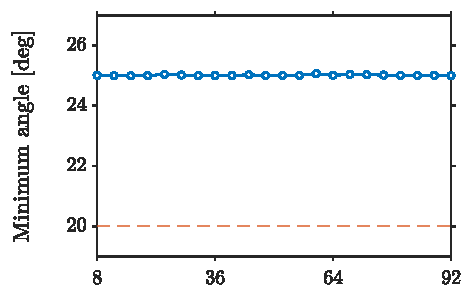
\includegraphics[width=\linewidth]{figures/quality/min_angle.pdf}
    \caption{Minimum triangle-angle check.}
    \label{fig:quality-angle}
  \end{subfigure}
  \hfill
  \begin{subfigure}[t]{0.485\linewidth}
    \centering
    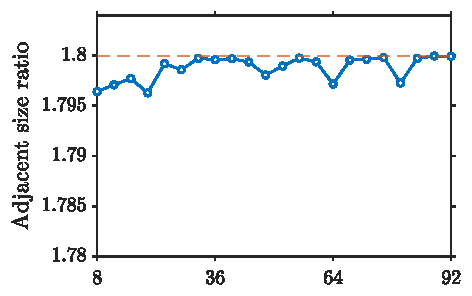
\includegraphics[width=\linewidth]{figures/quality/size_ratio.pdf}
    \caption{Adjacent element-size-ratio check.}
    \label{fig:quality-ratio}
  \end{subfigure}

  \medskip

  \begin{subfigure}[t]{0.485\linewidth}
    \centering
    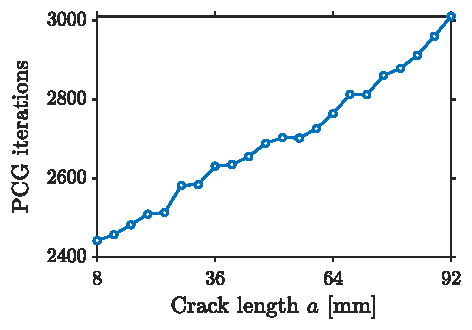
\includegraphics[width=\linewidth]{figures/quality/iterations.pdf}
    \caption{PCG iterations for accepted physical solves.}
    \label{fig:quality-iterations}
  \end{subfigure}
  \hfill
  \begin{subfigure}[t]{0.485\linewidth}
    \centering
    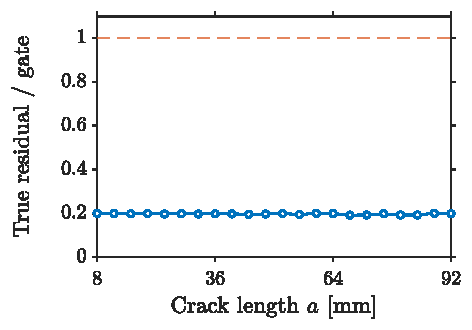
\includegraphics[width=\linewidth]{figures/quality/true_residual.pdf}
    \caption{True relative residual normalized by its acceptance gate.}
    \label{fig:quality-residual}
  \end{subfigure}

  \end{minipage}
  \caption{Diagnostics for accepted $P_2$--$P_{23}$ states. Dashed lines are
  the $20^\circ$ minimum-angle gate, 1.8 adjacent-size-ratio gate, and normalized
  true-residual gate of one. The separately enforced reported-PCG tolerance
  is $10^{-10}$; the true-residual acceptance denominator is
  $5\times10^{-10}$. No failed $P_{24}$ solve is plotted.}
  \label{fig:quality}
\end{figure}

\FloatBarrier
% The sn-mathphys-num class option selects sn-mathphys-num.bst automatically.
\bibliography{../../references}

% EDITORIAL HOLD: data/code availability and responsible AI-use disclosures
% still require author-approved wording before submission. Funding and competing
% interests have been confirmed and are included above.

\end{document}
